\documentclass[12pt]{article}

\usepackage[margin=1in]{geometry}
\usepackage[T1]{fontenc}
\usepackage[utf8]{inputenc}
\usepackage{amsmath,amssymb,bm,graphicx,physics}
\usepackage{authblk}
\usepackage{setspace}
\usepackage{caption}
\usepackage[hidelinks]{hyperref}

\graphicspath{{figures/supplementary/}{figures/main/}{./}}
\setstretch{1.15}

\title{Supplementary Information:\\
Programmable Quantum Resource Manifolds via Entanglement-Dynamic Topology}

\author[1]{Hang Hu \thanks{Correspondence to: hang.hu@cnrc-nrc.gc.ca}}
\affil[1]{Digital Technologies, National Research Council of Canada, 222 College Street, Toronto, ON M5T 3J1, Canada}
\author[1]{Hsu Kiang Ooi}
\author[2]{Anguang Hu \thanks{Correspondence to: anguang.hu@forces.gc.ca}}
\affil[2]{Suffield Research Centre, Defence Research and Development Canada, PO Box 4000 Station Main, Medicine Hat, Alberta T1A 8K6, Canada}

\date{\today}

\begin{document}

\maketitle

\section*{Overview}

This combined Supplementary Information accompanies the main-v4 manuscript,
\emph{Programmable Quantum Resource Manifolds via Entanglement-Dynamic Topology}.
It merges the concise Overleaf supplement with the extended local SI material atlas.
The central microscopic quantity is the curvature of electronic energies with respect
to a phonon normal-mode coordinate,
\begin{equation}
\kappa_{n\alpha}(k)=
\frac{\partial^2 E_n(k,Q_\alpha)}{\partial Q_\alpha^2},
\end{equation}
which captures the momentum-resolved second-order response of electronic structure
to lattice motion. This curvature encodes non-adiabatic electron--phonon coupling
and becomes strongly structured near degeneracies, where electronic states form
coupled resource manifolds~\cite{Giustino2017,Yarkony1996}.

\section*{S1. Curvature Derivation and Calculation Protocol}

Starting from the electron--phonon Hamiltonian,
\begin{equation}
H = H_e(\mathbf{r};\{Q_\alpha\}) +
\sum_\alpha
\left(
\frac{P_\alpha^2}{2M_\alpha}
+
\frac{1}{2}M_\alpha\omega_\alpha^2 Q_\alpha^2
\right),
\end{equation}
expanding the electronic Hamiltonian to second order in the normal-mode coordinates gives
\begin{equation}
H_e(\{Q_\alpha\})
\approx
H_e^{(0)}
+
\sum_\alpha Q_\alpha \partial_\alpha H_e
+
\frac{1}{2}\sum_{\alpha\beta}
Q_\alpha Q_\beta \partial_\alpha\partial_\beta H_e .
\end{equation}
Projection onto an adiabatic electronic basis introduces non-adiabatic coupling
terms (NACTs),
\begin{equation}
A_{mn}^{(\alpha)}=\langle m|\partial_{Q_\alpha}|n\rangle,
\end{equation}
which generate off-diagonal mixing and geometric phases~\cite{Mead1979,Berry1984}.

Electronic structure and electron--vibration interactions were computed using
all-electron quantum solid-state methods with numerical atomic orbitals, with
additional cross-checks against plane-wave density-functional calculations
where available~\cite{Blum2009,FHIaims2020,Giannozzi2009,Giannozzi2017}.
For each selected phonon normal mode $Q_\alpha$, band energies were recalculated
for symmetric positive and negative static displacements around the equilibrium
geometry. Second-order derivatives were evaluated using the five-point finite
difference stencil
\begin{equation}
\frac{\partial^2 A}{\partial u_\nu^2}
\approx
\frac{-A(-2\Delta u)+16A(-\Delta u)-30A(0)+16A(\Delta u)-A(2\Delta u)}
{12(\Delta u)^2}.
\end{equation}
The plotted traces are therefore momentum resolved, but the derivative is taken
with respect to the lattice normal-mode coordinate.

Near a quasi-degenerate two-band subspace $\{|i\rangle,|j\rangle\}$, the leading
interband-mixing contribution has the perturbative form
\begin{align}
\left.\frac{\partial^2 E_i}{\partial Q_\alpha^2}\right|_{\rm mix}
&\approx
+\frac{2|g_{ij}^{(\alpha)}(k)|^2}{\Delta_{ij}(k)},\\
\left.\frac{\partial^2 E_j}{\partial Q_\alpha^2}\right|_{\rm mix}
&\approx
-\frac{2|g_{ij}^{(\alpha)}(k)|^2}{\Delta_{ij}(k)},
\end{align}
where $\Delta_{ij}(k)=E_i(k)-E_j(k)$ and
$g_{ij}^{(\alpha)}(k)=\langle i|\partial H/\partial Q_\alpha|j\rangle$.
The equal-and-opposite signs express trace conservation within the local
two-level subspace. The associated NACT is
\begin{equation}
A_{ij}^{(\alpha)}(k)
=
\left\langle i\middle|\partial_{Q_\alpha}\middle|j\right\rangle
=
\frac{g_{ij}^{(\alpha)}(k)}{E_j(k)-E_i(k)},\qquad i\neq j,
\end{equation}
so curvature peaks are expected where the local gap is small and symmetry allows
the selected mode to couple the partner branches.

For the alkali-metal reference workflow~\cite{Hu2026_JPCM}, longitudinal modes
along symmetry-selected directions produced the strongest antisymmetric curvature
response, while transverse or mixed-polarized modes generally produced weaker
and more symmetric modulation. In the present EDT analysis, paired sign-opposite
curvature branches are treated as evidence of local non-adiabatic mixing, and
the subsequent window extraction tests whether that mixing remains smooth enough
to support a finite quadratic manifold.

When a displacement amplitude is needed to convert curvature into an energy
modulation, the second-order correction is
\begin{equation}
\Delta E_n(k)
\approx
\frac{1}{2}\kappa_{n\alpha}(k)(\Delta Q_\alpha)^2 .
\end{equation}
For zero-point or low-temperature estimates, $\Delta Q_\alpha$ may be obtained
from the Debye--Waller amplitude or the corresponding harmonic-oscillator
normal-mode amplitude~\cite{Ziman1972,AshcroftMermin}. The archived K$_3$C$_{60}$
workflow used here starts from already-computed curvature traces, so the
finite-window analysis does not reconstruct the displaced geometries.

\section*{S2. EDT Window Algorithm and K$_3$C$_{60}$ Details}

Paired curvature branches near crossings are fit locally to
\begin{equation}
\kappa_\pm(k)\approx a_\pm(k-k_0)^2+b_\pm .
\end{equation}
The EDT window $\Delta k_{\mathrm{EDT}}$ is defined as the interval over which
the local quadratic residual remains below a prescribed threshold. This gives a
reproducible, data-driven criterion for identifying finite structured manifolds.

The K$_3$C$_{60}$ case study combines an archived near-Fermi band-context figure
with an archived mode-resolved second-order band-curvature dataset. The
companion K$_3$C$_{60}$ figure identifies the representative phonon mode as
\texttt{m120} at $1090.35~\mathrm{cm}^{-1}$. The file
\texttt{data/k3c60/tmp.agr} is not a raw band-energy export; it stores the
already-evaluated second-order band-curvature traces
$\partial^2 E_n(k,Q_\alpha)/\partial Q_\alpha^2$ for many band indices along
the $\Gamma$--X--L--W--$\Gamma$ path. The embedded Grace metadata provide the
path labels, dataset legends, and the plotted curvature quantity, so the finite
window extraction starts directly from archived curvature data rather than from
reconstructing displaced geometries or re-differentiating energies.

The curvature-window analysis shown in the main-text K$_3$C$_{60}$ figure and
in Fig.~\ref{fig:s5_threshold_bootstrap} is implemented explicitly in
\texttt{scripts/make\_fig2\_k3c60\_edt.py}. The script first parses the AGR file
into individual band-curvature datasets and reads the embedded legends to map
dataset numbers to archived band labels. It then selects datasets 207 and 208,
corresponding to archived Bands 208 and 209, and restricts the analysis to the
momentum slice indexed from 150 to 281, which isolates the local crossing
region used in the main-text figure. Within that slice, the negative branch is
centered by its local minimum and the positive branch by its local maximum.
Around each extremum, the script extracts a symmetric fitting neighborhood of
18 points on either side and performs an independent quadratic fit to each
branch.

Those fitted parabolas are then evaluated over the full selected momentum
slice, and branchwise normalized residuals are computed as the absolute
deviation between the archived curvature trace and the fitted quadratic, scaled
by the maximum branch amplitude in the same slice. Using the nominal threshold
$R_{\rm th}=0.08$, the script identifies the contiguous below-threshold region
connected to each branch extremum. The reported EDT window
$\Delta k_{\mathrm{EDT}}$ is defined as the union of those two contiguous
regions, while the tighter core region is taken as their overlap whenever that
overlap is nonempty. The same script also generates the robustness scans by
varying the residual threshold, the local fit half-window, neighboring band
pairs, and the effective $k$-grid density, and it estimates uncertainty by
bootstrap resampling of the local fit points before recomputing the window
width.

\section*{S3. Expanded Curvature-Manifold Materials Study}

We extend the K$_3$C$_{60}$ curvature-window workflow to elemental V, elemental
Na, LaH$_{10}$, and YBa$_2$Cu$_3$O$_7$ using the same paired-curvature, local
quadratic-fit, residual-threshold, and bootstrap procedure used for Fig.~2 in
the main text. These datasets span a transition metal, a simple metal, a
high-pressure hydride, and a correlated oxide. The resulting figures should be
read as replicated curvature-manifold analyses on representative archived branch
pairs rather than exhaustive mode scans, but they place all materials on a
common diagnostic footing and make the finite-window structure directly
comparable.

\begin{figure}[p]
\centering
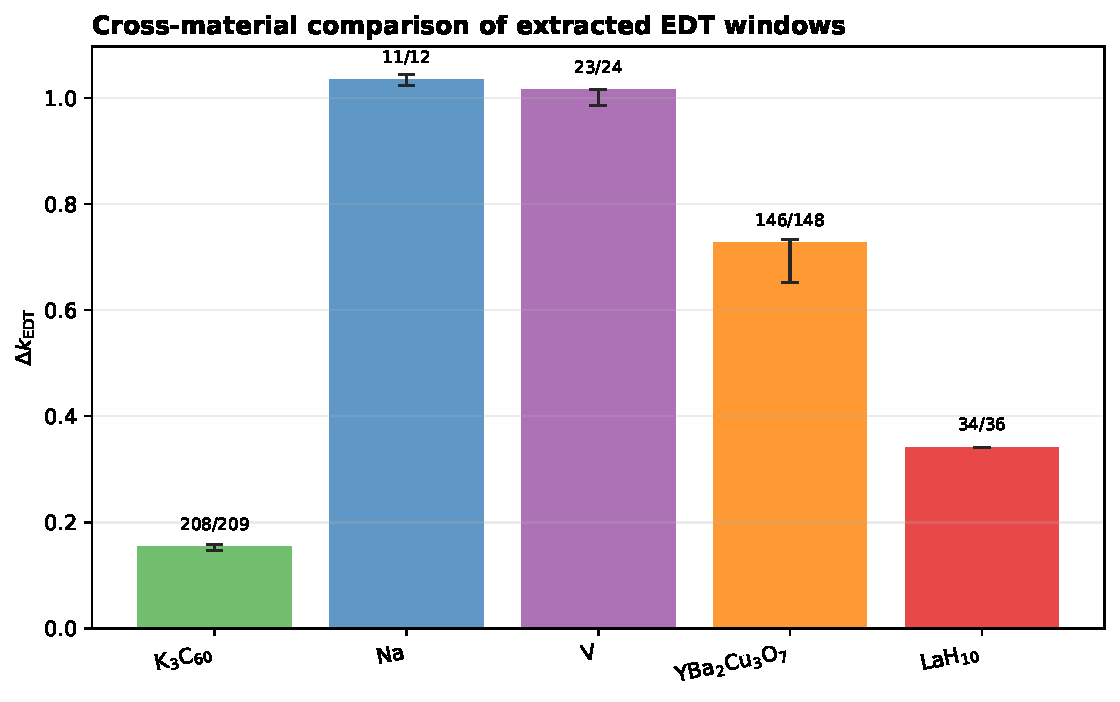
\includegraphics[width=0.78\linewidth]{S3_material_summary.pdf}
\caption{\textbf{Cross-material summary of extracted EDT-window widths.}
The bar heights show the residual-defined $\Delta k_{\mathrm{EDT}}$ values
extracted from the selected representative branch pairs in K$_3$C$_{60}$, Na,
V, YBa$_2$Cu$_3$O$_7$, and LaH$_{10}$, while the error bars show bootstrap
confidence intervals from the local quadratic-fit procedure. This compact
summary is the supplementary overview of the branch-resolved analyses shown in
the figures below and highlights that the same curvature-window diagnostic does
not produce one universal window scale across materials.}
\label{fig:s4_material_controls}
\end{figure}

\begin{table}[p]
\centering
\small
\caption{Representative branch-pair results extracted from the expanded
curvature-manifold workflow at the
common residual threshold $R_{\rm th}=0.08$. Widths are reported in the native
$k$ coordinate of each archived export, and the bootstrap interval corresponds
to the 95\% width confidence range from the replicated local fit.}
\begin{tabular}{lllll}
\hline
Material & Pair & $k_0$ & $\Delta k_{\mathrm{EDT}}$ & Bootstrap 95\% CI \\
\hline
K$_3$C$_{60}$ & 208/209 & 0.823 & 0.154 & [0.147, 0.158] \\
V & 22/23 & 2.718 & 1.016 & [0.986, 1.016] \\
Na & 11/12 & 1.837 & 1.035 & [1.024, 1.045] \\
YBa$_2$Cu$_3$O$_7$ & 145/147 subset & 1.599 & 0.727 & [0.652, 0.733] \\
LaH$_{10}$ & 33/35 subset & 1.300 & 0.342 & [0.342, 0.342] \\
\hline
\end{tabular}
\label{tab:s4_material_controls}
\end{table}

The extended material atlas now replicates the curvature-manifold
workflow for the archived materials cases. For each material we show the band
context, the selected paired curvature branches, the local quadratic fit, the
residual-defined EDT window, and the threshold/bootstrap summary generated with
the same paired-curvature and residual-threshold procedure used in the main-text
K$_3$C$_{60}$ analysis. Taken together, these figures show that the same
diagnostic can return broad, intermediate, or sharply localized finite windows
depending on how smoothly the selected branch pair sustains a local quadratic
manifold.

The cross-material trends are already informative at the representative-pair
level. V still exhibits the broadest extracted window, indicating that the
selected branch pair maintains a smooth quadratic compatibility over a
comparatively large momentum interval. With the updated pair choice, Na now
provides a much broader simple-metal baseline through Bands 11 and 12, rather
than the narrower nonadjacent pairing used previously. For the updated
YBa$_2$Cu$_3$O$_7$ and LaH$_{10}$ selections, the relevant curvature
organization survives only over a more localized region of momentum space. In
practical terms, the expanded atlas supports the conclusion that EDT-like
structure is reproducible across multiple materials, but its width and
robustness are strongly material and branch dependent.

Figure~\ref{fig:s4_material_controls} is useful as a first summary because it
separates two effects that are otherwise easy to mix together. The bar heights
compare the nominal extracted window sizes, whereas the error bars quantify how
stable those widths remain under bootstrap refitting of the local branch
structure. In the present representative selections, K$_3$C$_{60}$ remains the
narrowest reference case, Na and V support broader metallic windows, and the
YBa$_2$Cu$_3$O$_7$ and LaH$_{10}$ subsets remain more localized. The panel does
not replace the branch-resolved figures below; instead, it tells the reader
how much of the comparison comes from genuine differences in extracted window
size and how much comes from uncertainty in the local quadratic fit.

\begin{figure}[p]
\centering
\begin{minipage}{0.48\linewidth}
\textbf{(a)}\\[-0.4em]
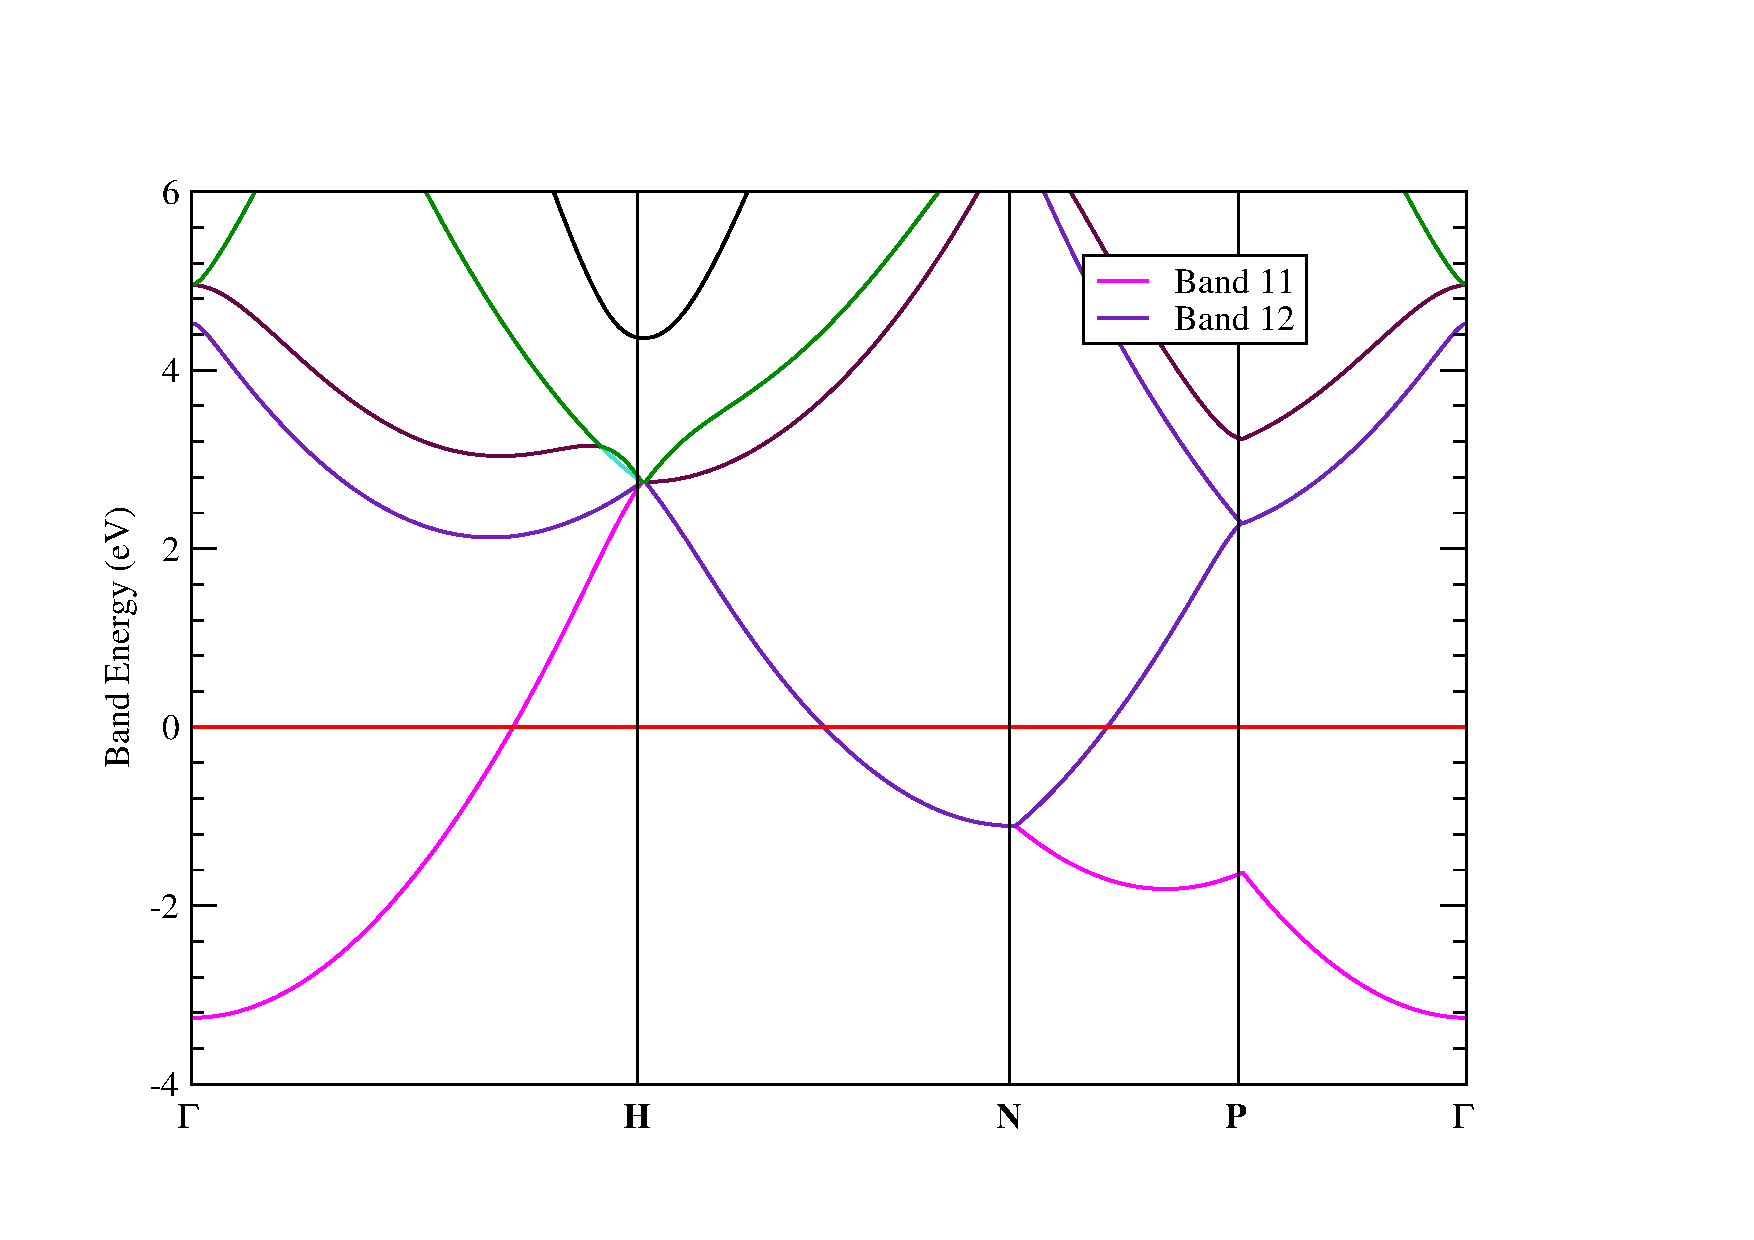
\includegraphics[width=\linewidth]{Na_bands.pdf}
\end{minipage}\hfill
\begin{minipage}{0.48\linewidth}
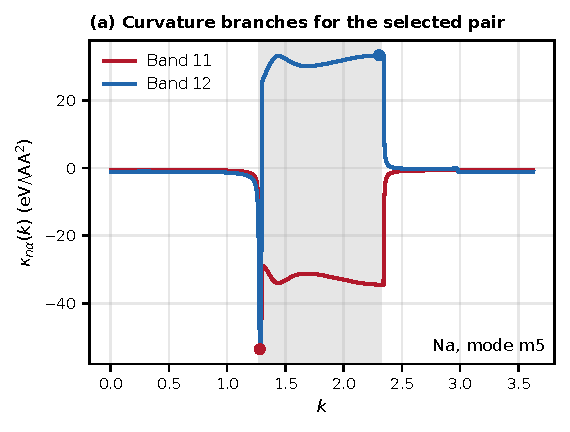
\includegraphics[width=\linewidth]{S1_Na_panel_b_curvature.pdf}
\end{minipage}

\vspace{0.5em}

\begin{minipage}{0.48\linewidth}
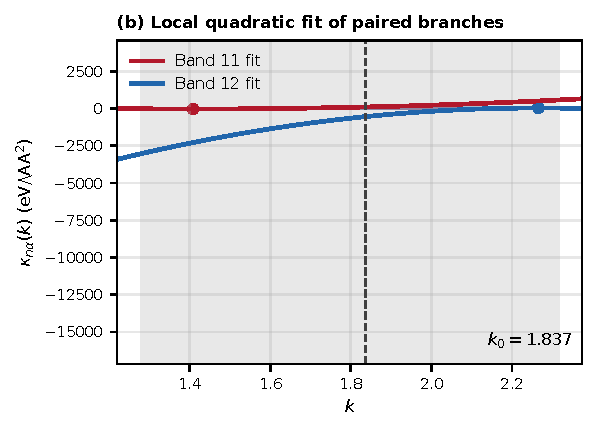
\includegraphics[width=\linewidth]{S1_Na_panel_c_fit.pdf}
\end{minipage}\hfill
\begin{minipage}{0.48\linewidth}
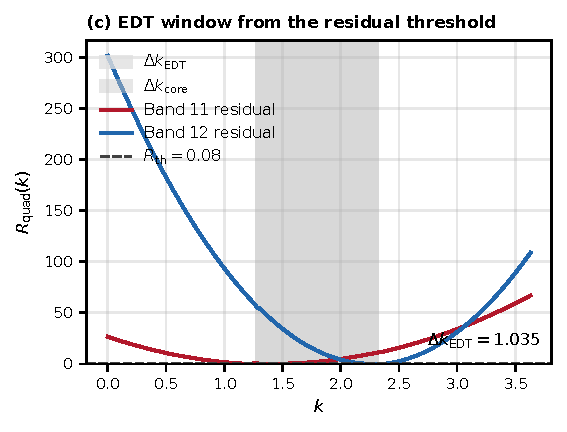
\includegraphics[width=\linewidth]{S1_Na_panel_d_window.pdf}
\end{minipage}

\vspace{0.5em}

\begin{minipage}{0.48\linewidth}
\centering
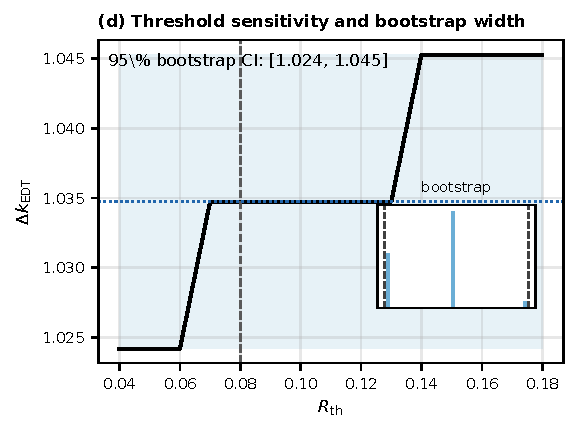
\includegraphics[width=\linewidth]{S1_Na_panel_e_bootstrap.pdf}
\end{minipage}
\caption{\textbf{Extended curvature-manifold analysis for Na.}
(a) Band-structure context for bcc Na. (b) Selected paired curvature branches
for the archived mode-resolved export. (c) Local quadratic fit of the paired
branches. (d) Residual-defined candidate EDT window at the common threshold
$R_{\rm th}=0.08$. (e) Threshold sensitivity and bootstrap width summary. Na
provides the simple-metal baseline for the expanded materials workflow using
Bands 11 and 12, with a representative window centered at
$k_0\approx 1.84$ and $\Delta k_{\mathrm{EDT}}\approx 1.035$.}
\label{fig:si_na}
\end{figure}

\begin{figure}[p]
\centering
\begin{minipage}{0.48\linewidth}
\textbf{(a)}\\[-0.4em]
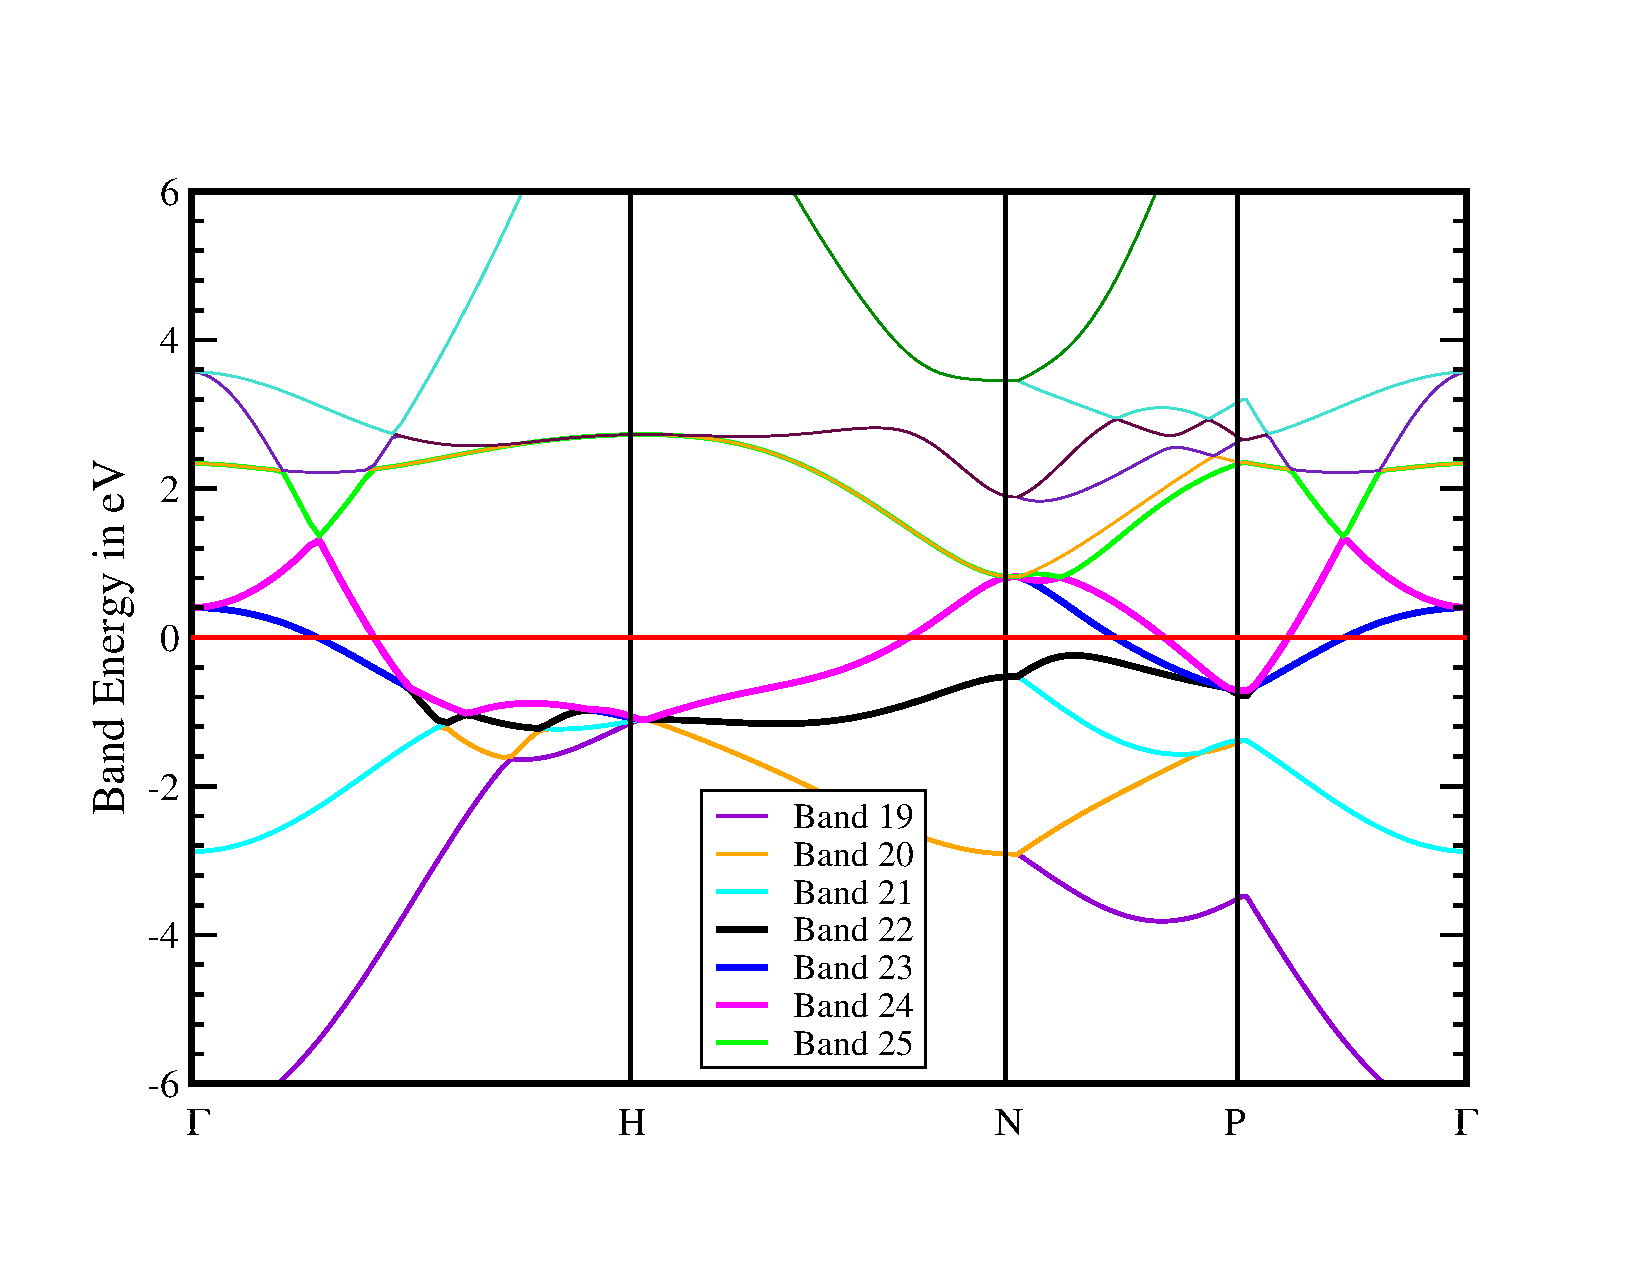
\includegraphics[width=\linewidth]{V-bands.pdf}
\end{minipage}\hfill
\begin{minipage}{0.48\linewidth}
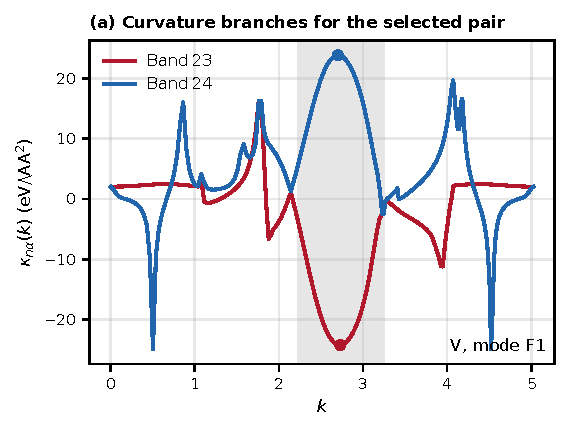
\includegraphics[width=\linewidth]{S2_V_panel_b_curvature.pdf}
\end{minipage}

\vspace{0.5em}

\begin{minipage}{0.48\linewidth}
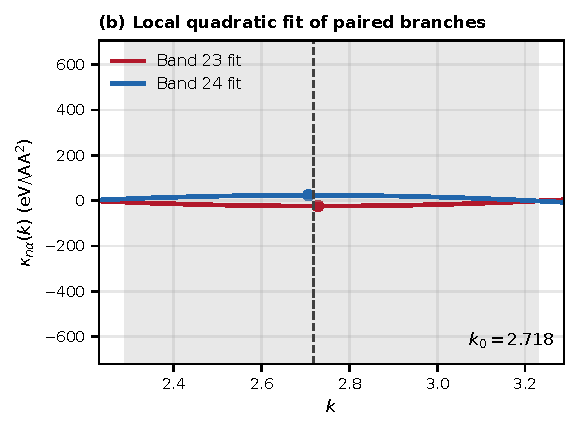
\includegraphics[width=\linewidth]{S2_V_panel_c_fit.pdf}
\end{minipage}\hfill
\begin{minipage}{0.48\linewidth}
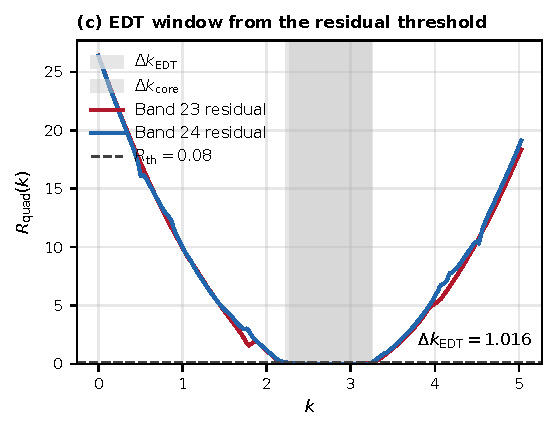
\includegraphics[width=\linewidth]{S2_V_panel_d_window.pdf}
\end{minipage}

\vspace{0.5em}

\begin{minipage}{0.48\linewidth}
\centering
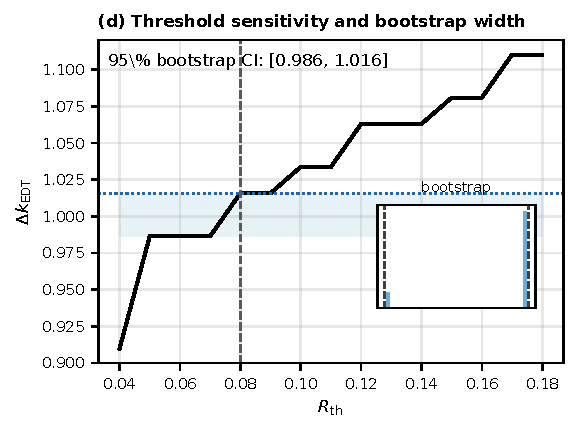
\includegraphics[width=\linewidth]{S2_V_panel_e_bootstrap.pdf}
\end{minipage}
\caption{\textbf{Extended curvature-manifold analysis for V.}
(a) Band-structure context for elemental V. (b) Selected paired curvature
branches for the archived mode-resolved export. (c) Local quadratic fit of the
paired branches. (d) Residual-defined candidate EDT window at the common
threshold $R_{\rm th}=0.08$. (e) Threshold sensitivity and bootstrap width
summary. V provides the broadest representative window in the expanded study,
with $k_0\approx 2.72$ and $\Delta k_{\mathrm{EDT}}\approx 1.02$.}
\label{fig:si_v}
\end{figure}

\begin{figure}[p]
\centering
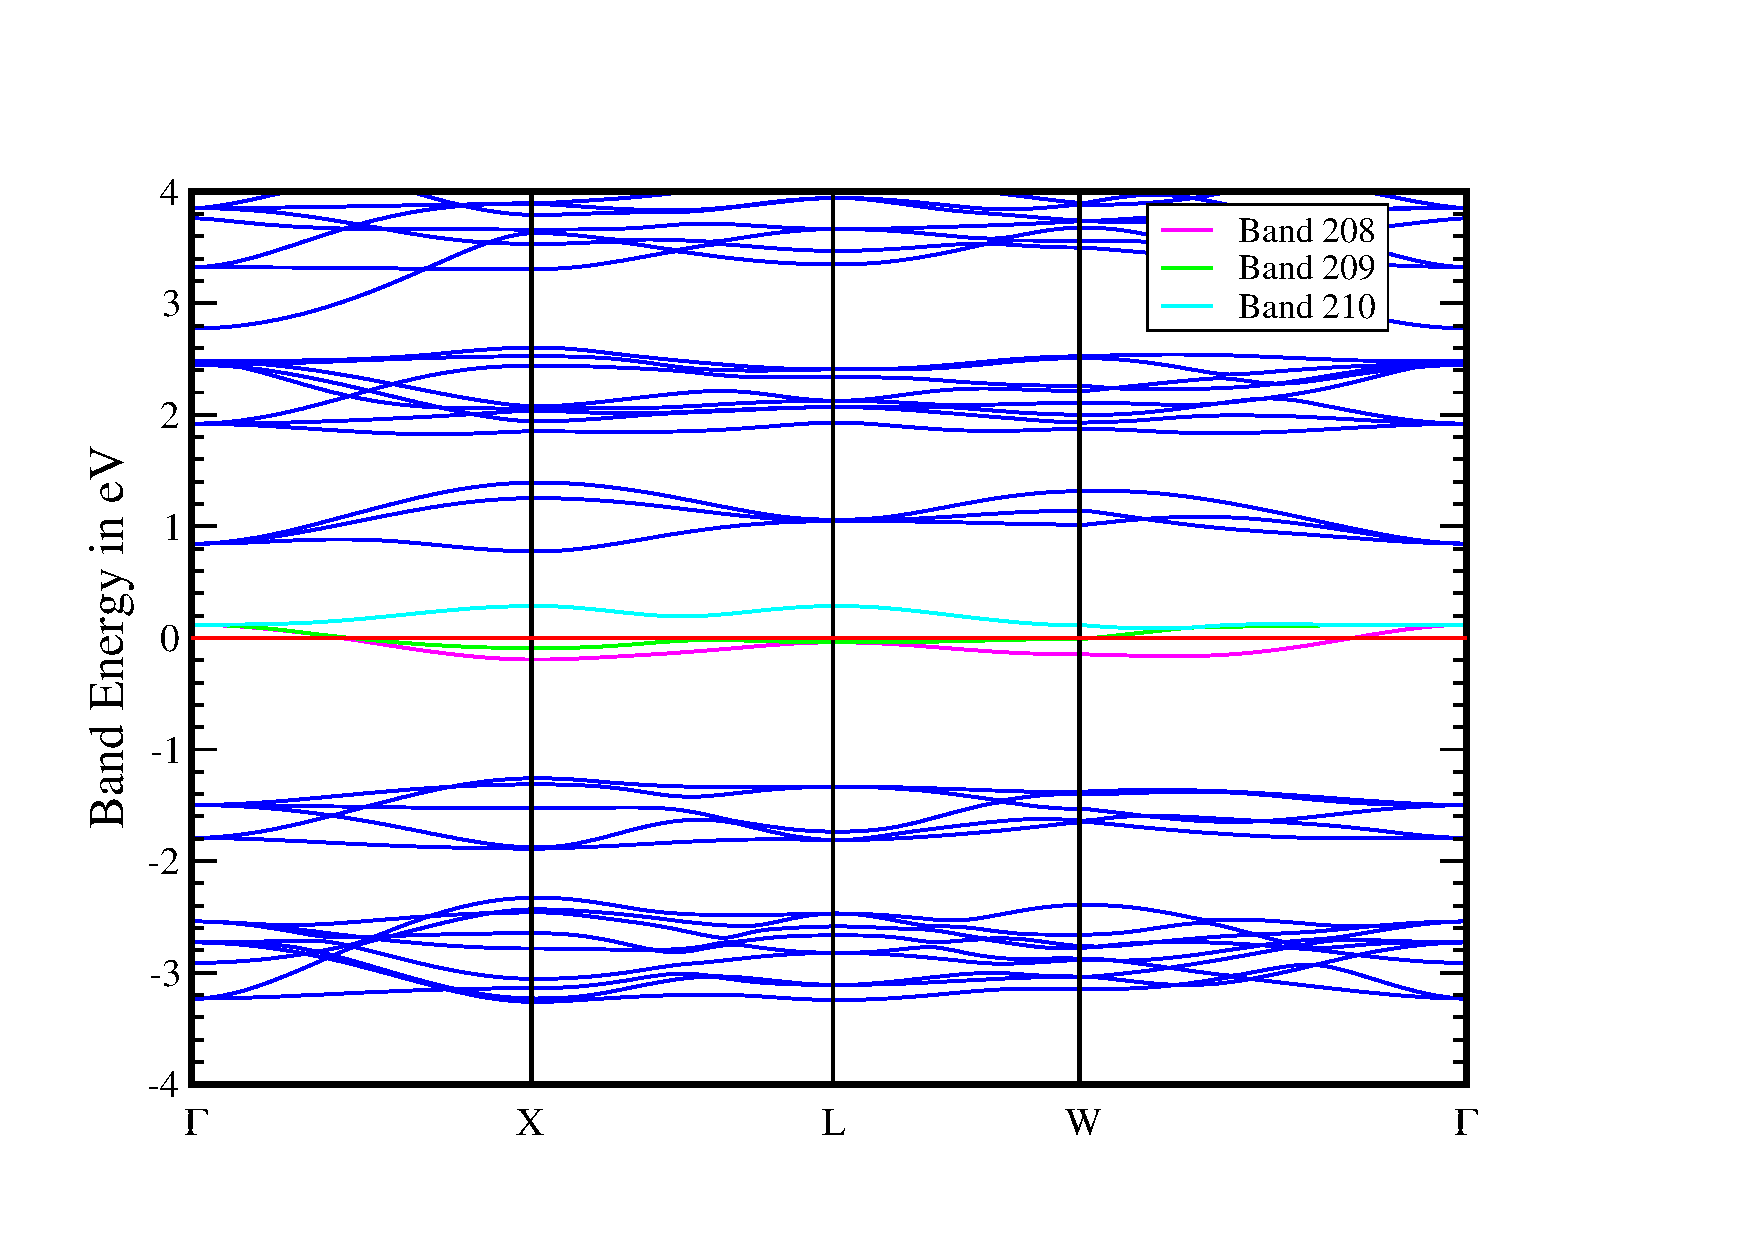
\includegraphics[width=0.78\textwidth]{K3C60-bands.pdf}
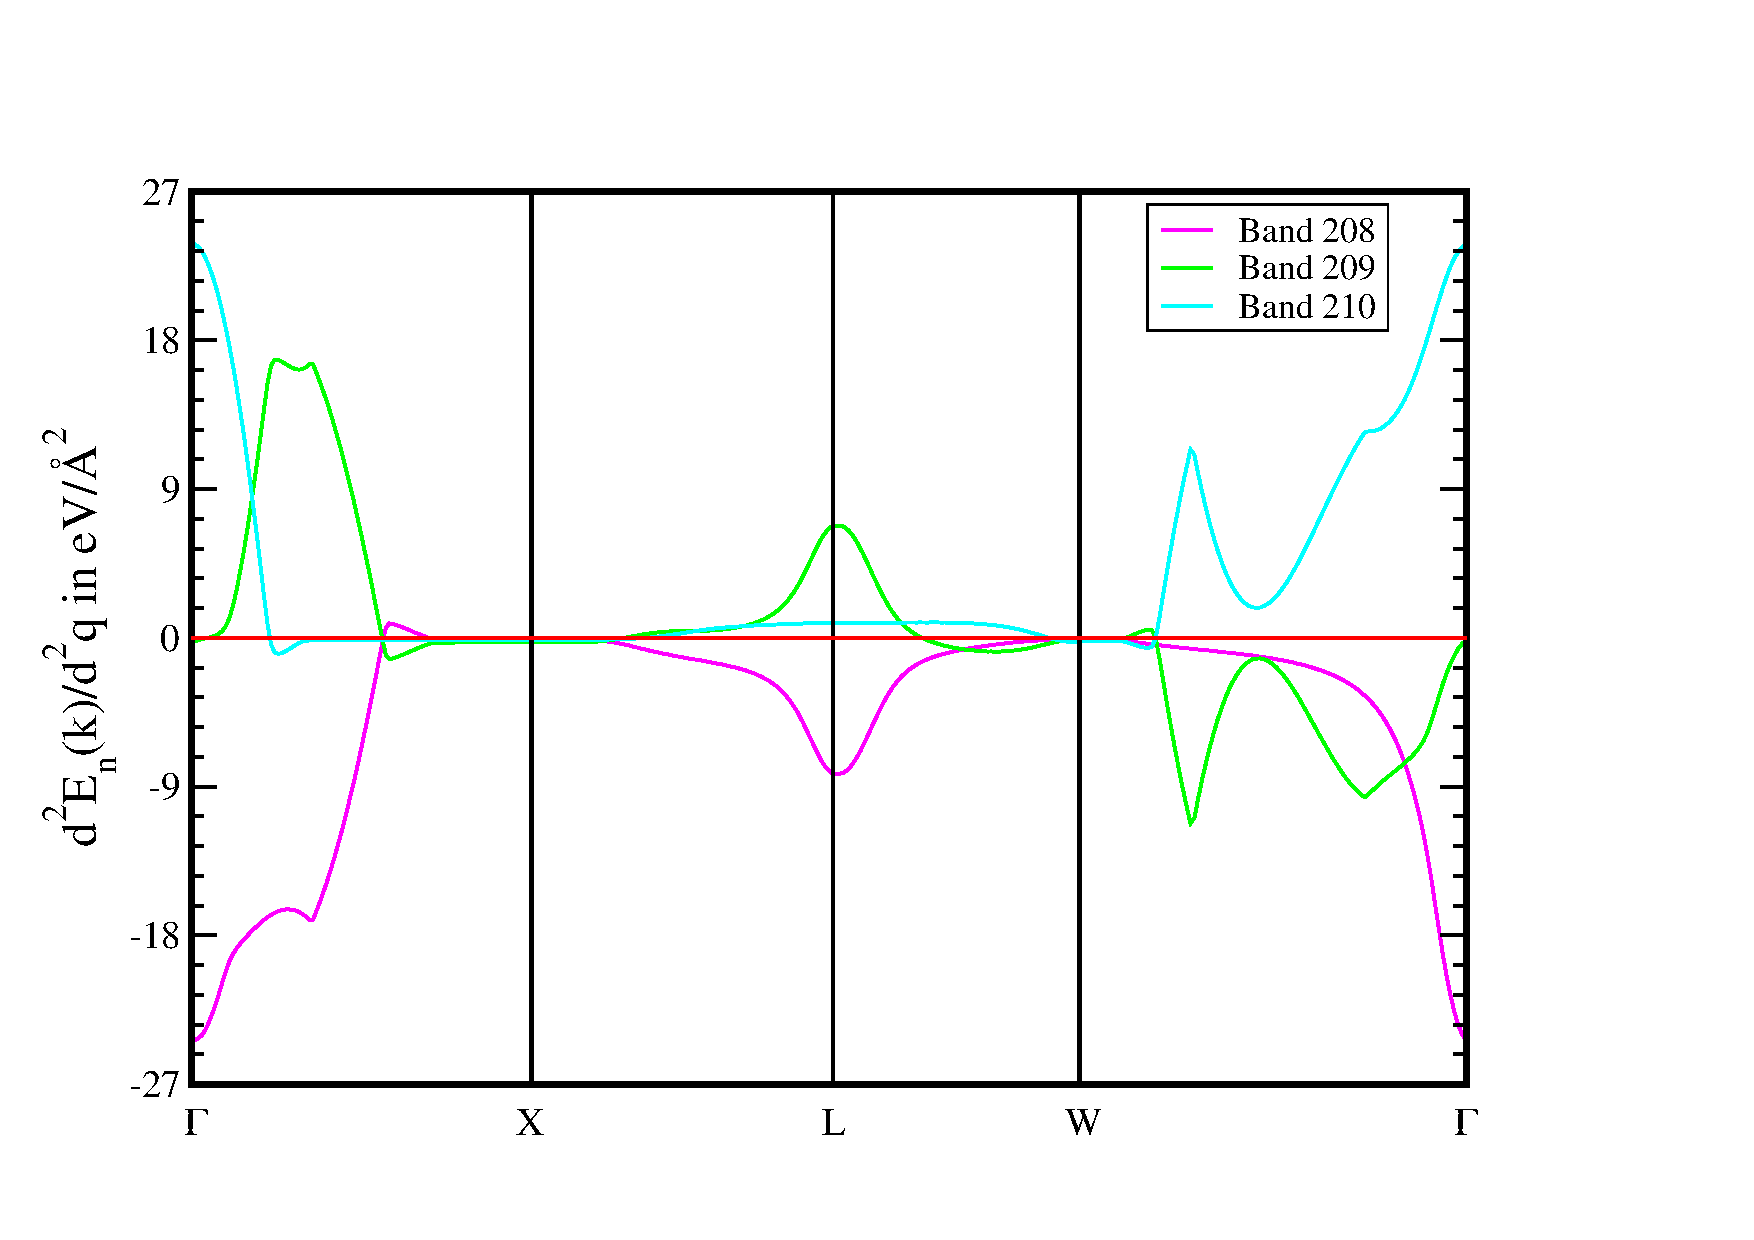
\includegraphics[width=0.78\textwidth]{K3C60-m120.pdf}
\caption{\textbf{Curvature-resolved electronic structure of K$_3$C$_{60}$.}
The near-Fermi band context and representative mode-resolved curvature export
show structured non-adiabatic electron--phonon response. This material provides
the main quantitative curvature-window example in the manuscript.}
\label{fig:si_k3c60}
\end{figure}

\begin{figure}[p]
\centering
\begin{minipage}{0.48\linewidth}
\textbf{(a)}\\[-0.4em]
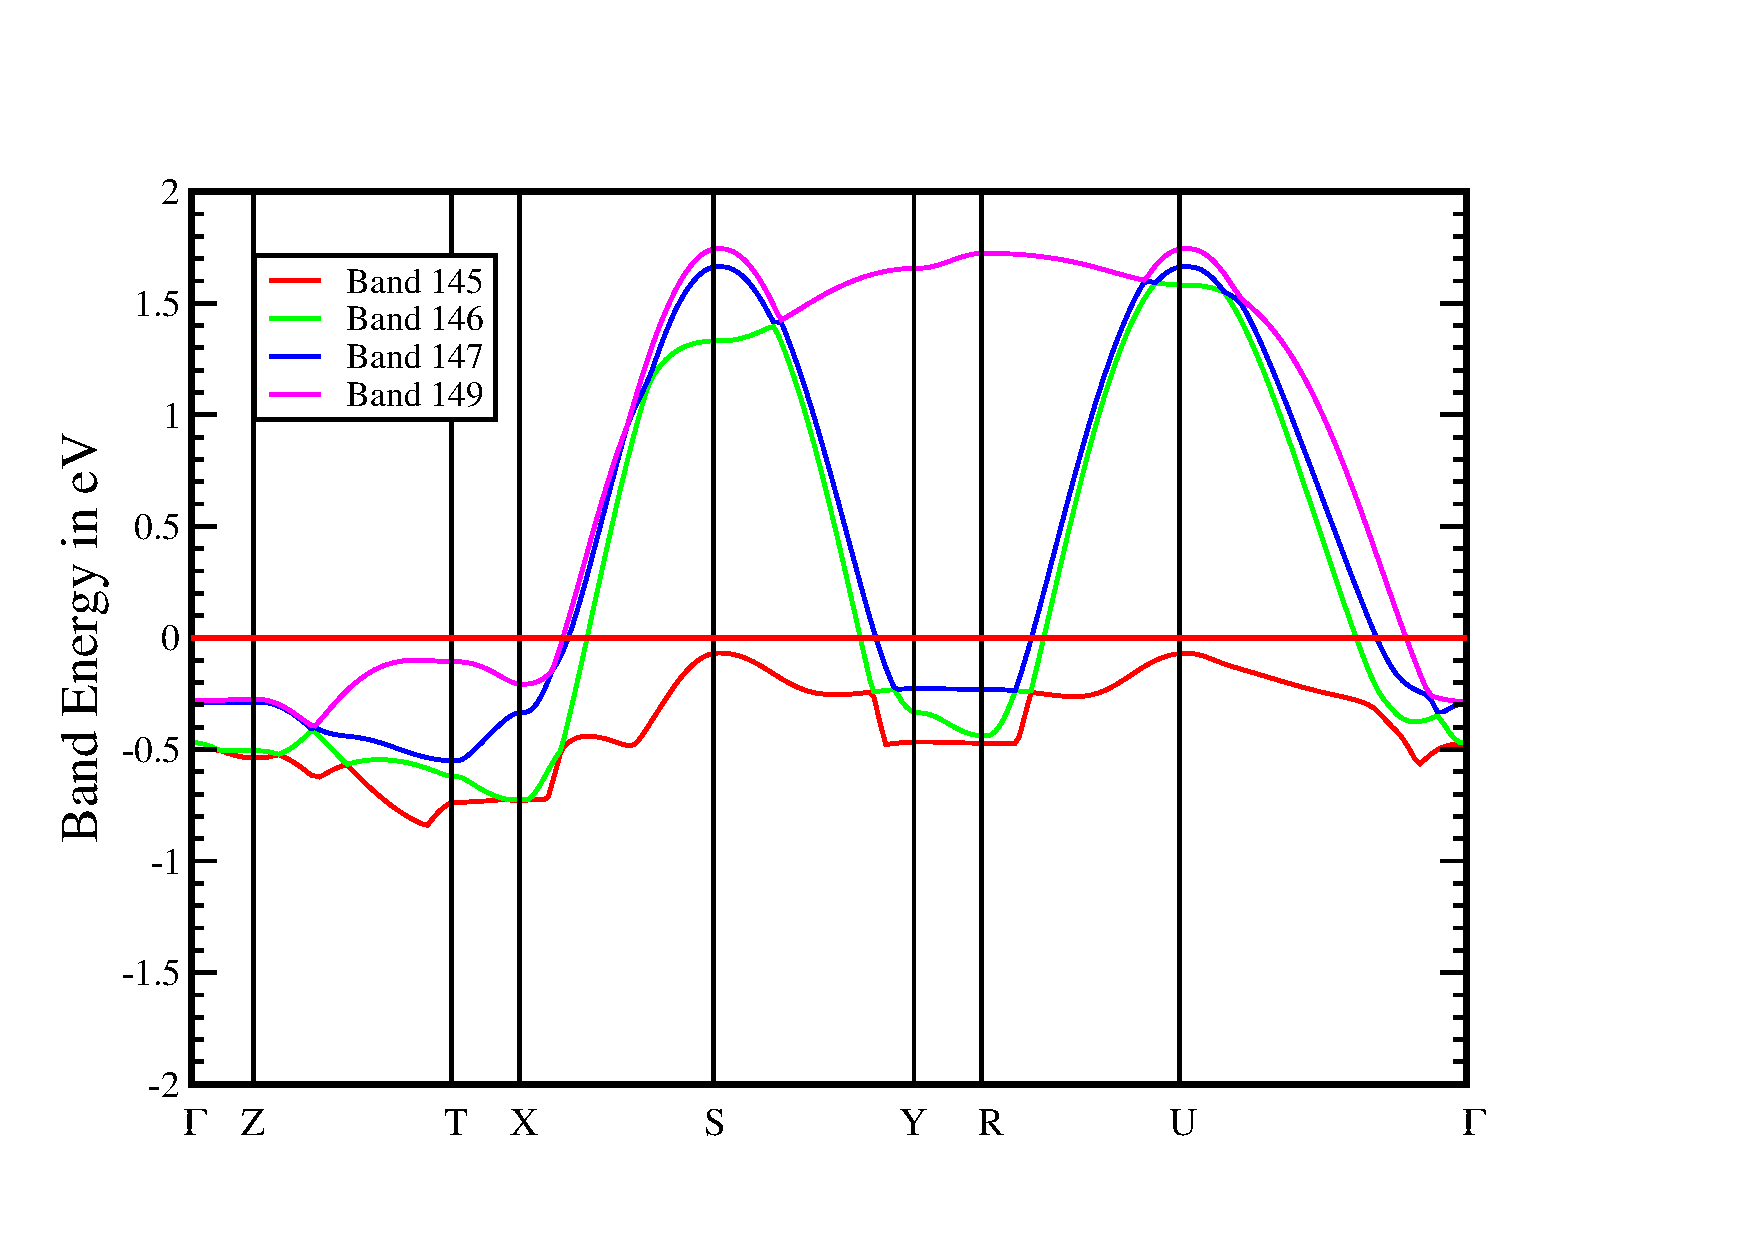
\includegraphics[width=\linewidth]{YBa2Cu3O7_bands.pdf}
\end{minipage}\hfill
\begin{minipage}{0.48\linewidth}
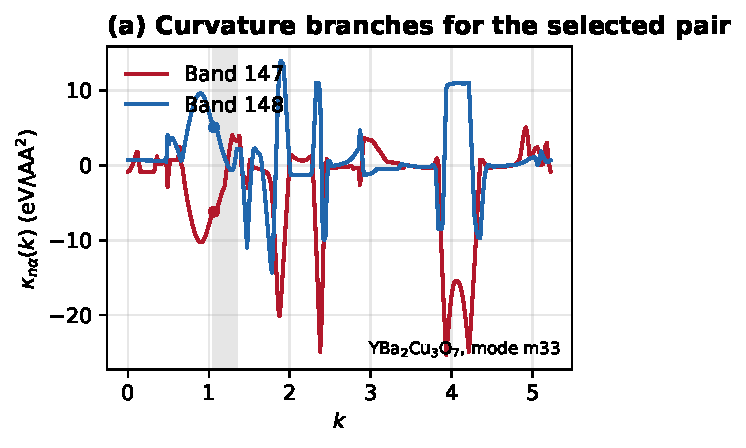
\includegraphics[width=\linewidth]{S4_YBa2Cu3O7_panel_b_curvature.pdf}
\end{minipage}

\vspace{0.5em}

\begin{minipage}{0.48\linewidth}
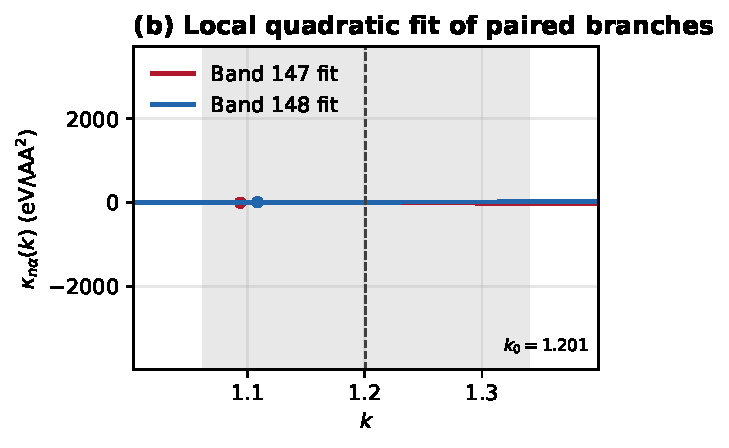
\includegraphics[width=\linewidth]{S4_YBa2Cu3O7_panel_c_fit.pdf}
\end{minipage}\hfill
\begin{minipage}{0.48\linewidth}
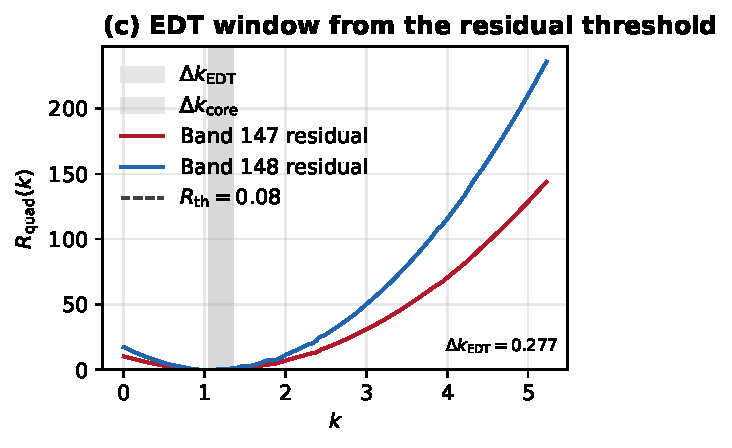
\includegraphics[width=\linewidth]{S4_YBa2Cu3O7_panel_d_window.pdf}
\end{minipage}

\vspace{0.5em}

\begin{minipage}{0.48\linewidth}
\centering
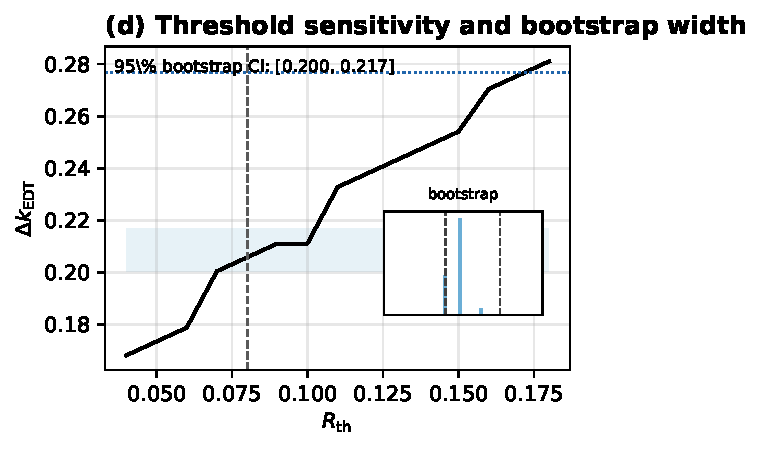
\includegraphics[width=\linewidth]{S4_YBa2Cu3O7_panel_e_bootstrap.pdf}
\end{minipage}
\caption{\textbf{Extended curvature-manifold analysis for YBa$_2$Cu$_3$O$_7$.}
(a) Band-structure context for YBa$_2$Cu$_3$O$_7$. (b) Selected paired curvature
branches for the archived mode-resolved export. (c) Local quadratic fit of the
paired branches. (d) Residual-defined candidate EDT window at the common
threshold $R_{\rm th}=0.08$. (e) Threshold sensitivity and bootstrap width
summary. The representative pair shown here is drawn from the requested
145/146/147/149 band subset and gives a localized window around
$k_0\approx 1.60$ with $\Delta k_{\mathrm{EDT}}\approx 0.727$.}
\label{fig:si_ybco}
\end{figure}

\begin{figure}[p]
\centering
\begin{minipage}{0.48\linewidth}
\textbf{(a)}\\[-0.4em]
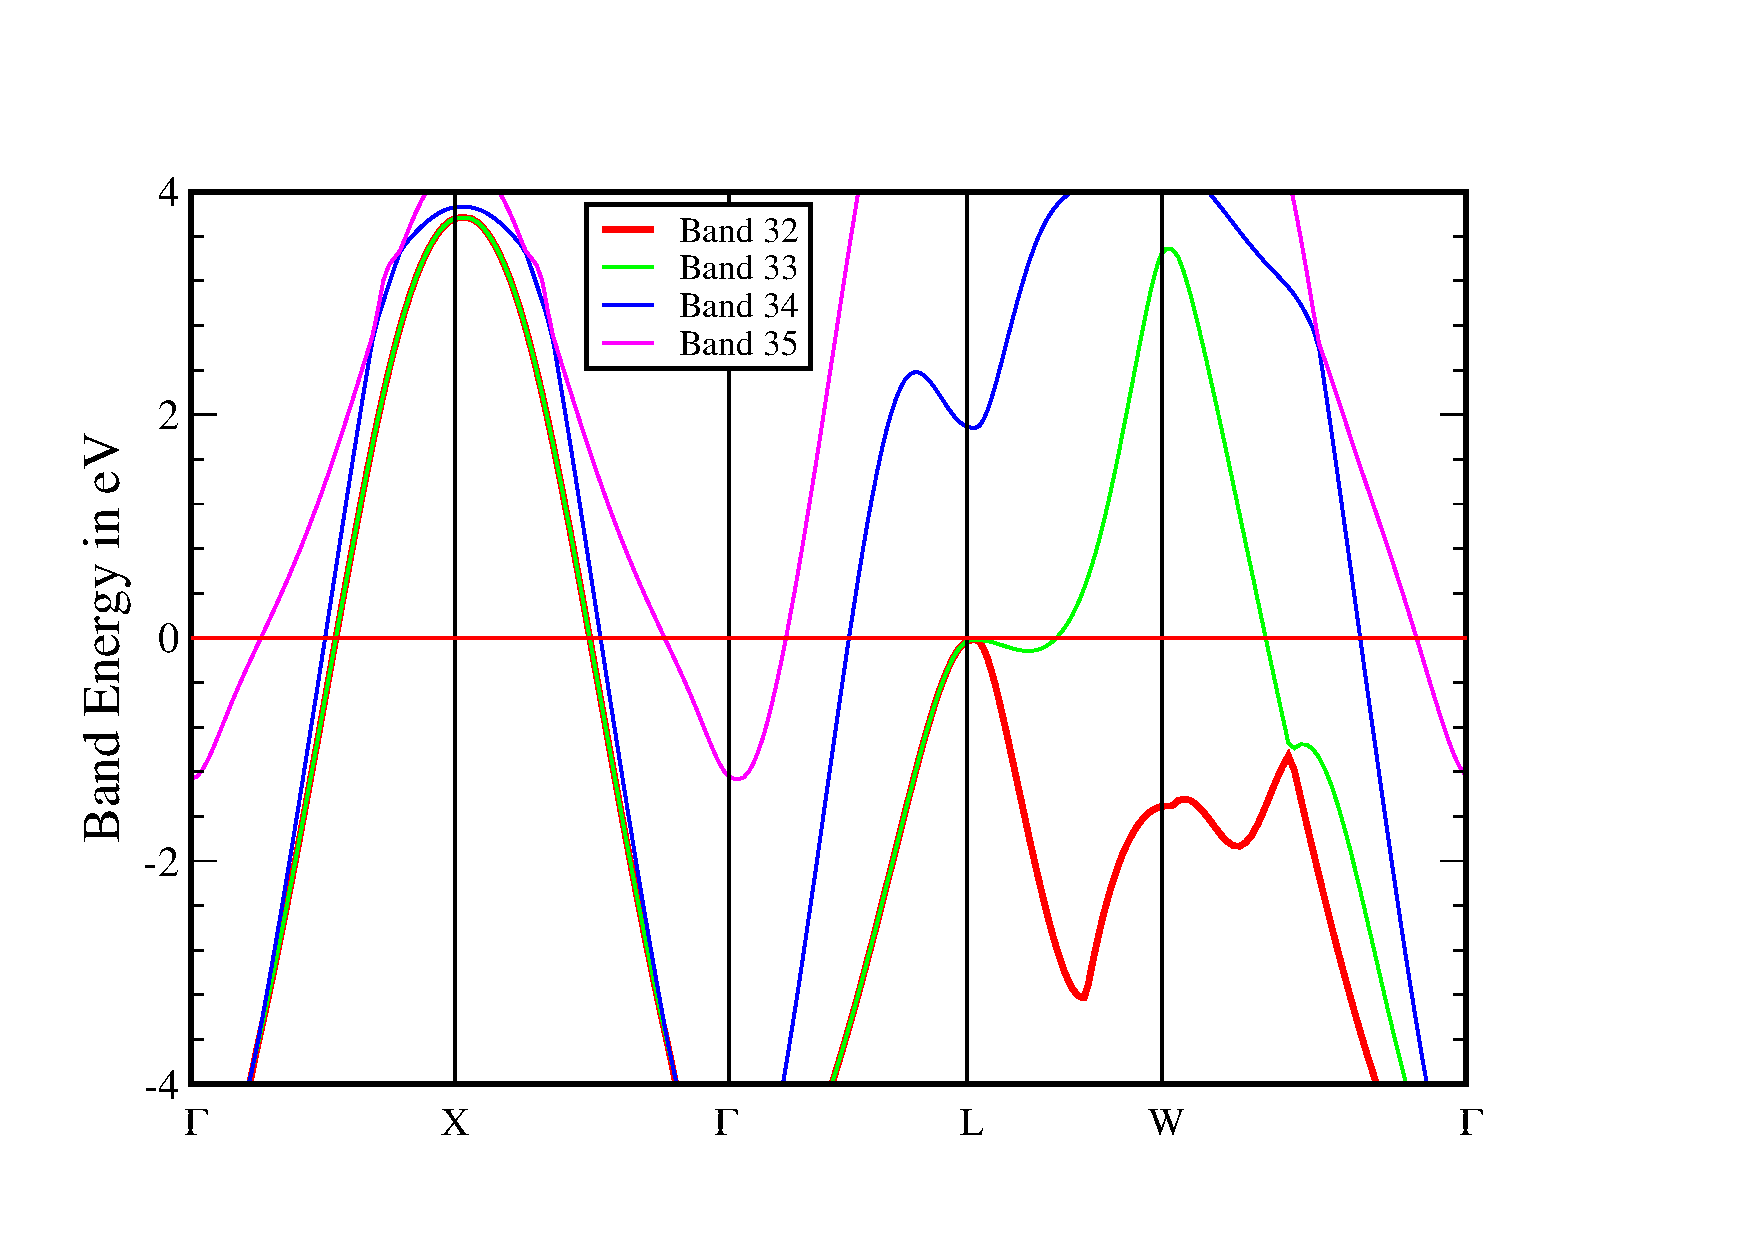
\includegraphics[width=\linewidth]{LaH10-300GPa-bands.pdf}
\end{minipage}\hfill
\begin{minipage}{0.48\linewidth}
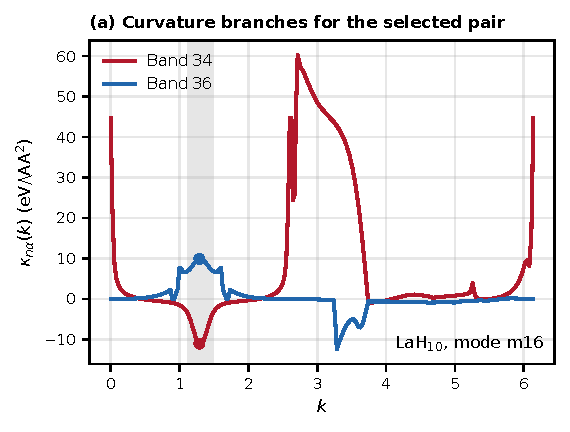
\includegraphics[width=\linewidth]{S5_LaH10_panel_b_curvature.pdf}
\end{minipage}

\vspace{0.5em}

\begin{minipage}{0.48\linewidth}
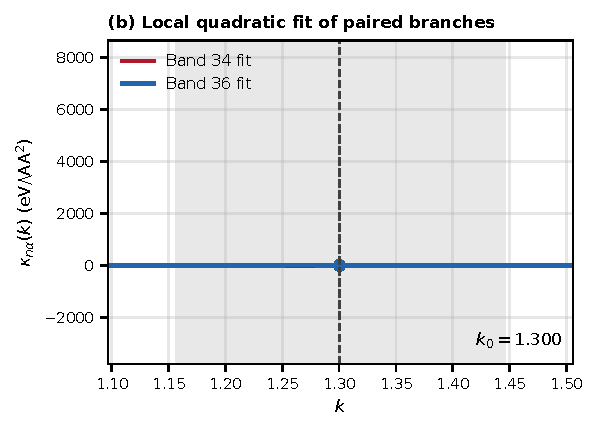
\includegraphics[width=\linewidth]{S5_LaH10_panel_c_fit.pdf}
\end{minipage}\hfill
\begin{minipage}{0.48\linewidth}
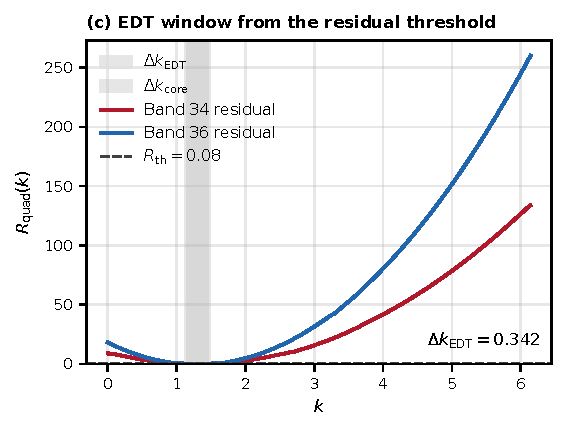
\includegraphics[width=\linewidth]{S5_LaH10_panel_d_window.pdf}
\end{minipage}

\vspace{0.5em}

\begin{minipage}{0.48\linewidth}
\centering
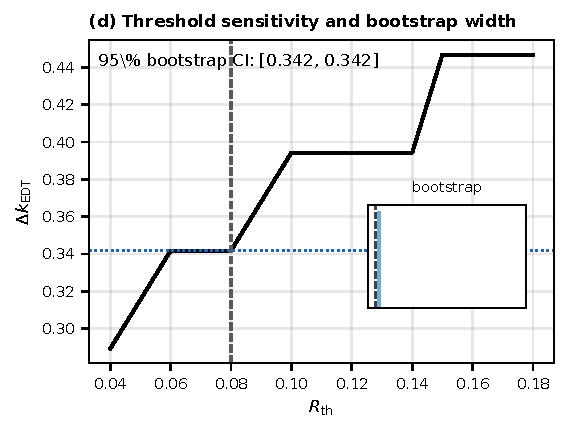
\includegraphics[width=\linewidth]{S5_LaH10_panel_e_bootstrap.pdf}
\end{minipage}
\caption{\textbf{Extended curvature-manifold analysis for LaH$_{10}$.}
(a) Band-structure context for LaH$_{10}$ at high pressure. (b) Selected paired
curvature branches for the archived mode-resolved export. (c) Local quadratic
fit of the paired branches. (d) Residual-defined candidate EDT window at the
common threshold $R_{\rm th}=0.08$. (e) Threshold sensitivity and bootstrap
width summary. The representative pair shown here is drawn from the 32--35 band
subset and yields a localized window near $k_0\approx 1.30$ with
$\Delta k_{\mathrm{EDT}}\approx 0.342$.}
\label{fig:si_lah10}
\end{figure}

\section*{S4. Threshold, Bootstrap, and Temperature Robustness}

Figure~\ref{fig:s5_threshold_bootstrap} collects the analysis variations used to
test the stability of the K$_3$C$_{60}$ curvature-defined EDT window. The
nominal configuration uses Bands 208 and 209 of mode \texttt{m120}, analysis
indices 150--281, local quadratic fit half-window of 18 points, and residual
threshold $R_{\rm th}=0.08$. The resulting nominal width is
$\Delta k_{\rm EDT}=0.154$.

A residual-threshold sweep over $R_{\rm th}\in[0.04,0.18]$ yields widths between
0.137 and 0.178. A fit-window sweep over half-windows from 10 to 28 points yields
widths between 0.127 and 0.199. A local-fit bootstrap around the nominal paired
branches gives a 95\% confidence interval of $[0.147,0.158]$ for the extracted
width. Subsampling the $k$ grid changes the width only modestly.

\begin{figure}[p]
\centering
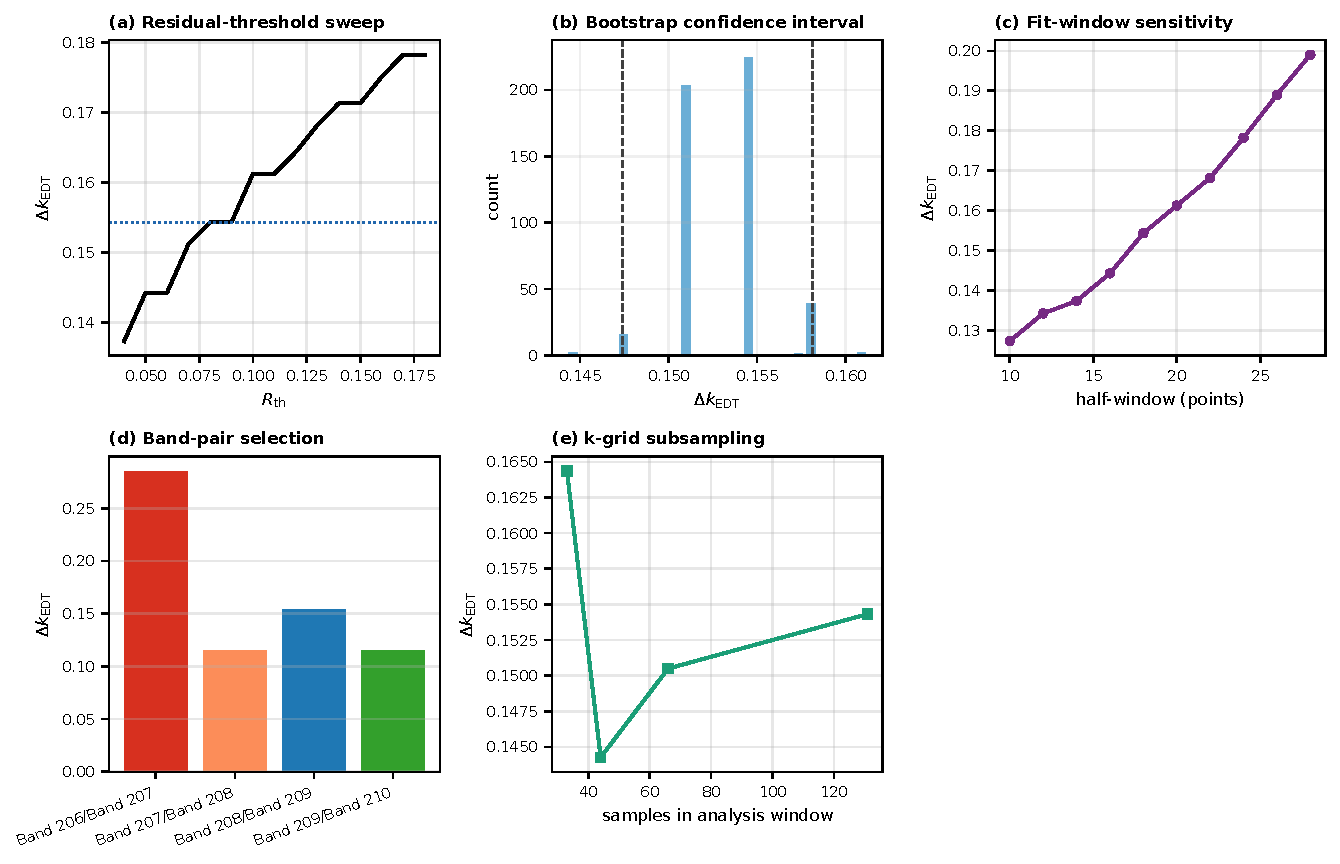
\includegraphics[width=0.95\linewidth]{S5_threshold_bootstrap.pdf}
\caption{\textbf{Robustness checks for the K$_3$C$_{60}$ curvature-defined EDT
window.} The panels summarize residual-threshold sensitivity, bootstrap
uncertainty, local-fit-window sensitivity, neighboring band-pair choices,
$k$-grid decimation, and the unavailable displacement-amplitude sweep in the
bundled archive.}
\label{fig:s5_threshold_bootstrap}
\end{figure}

Temperature-dependent band structures are treated as a dynamical probe of
NACT-induced geometry. In EDT-compatible systems such as Nb, temperature-induced
renormalization preserves band connectivity and near-degenerate structure,
maintaining paired smooth curvature profiles. In sharper systems, temperature
can enhance nonuniform degeneracy lifting and reduce the stability of a local
quadratic description.

\begin{figure}[p]
\centering
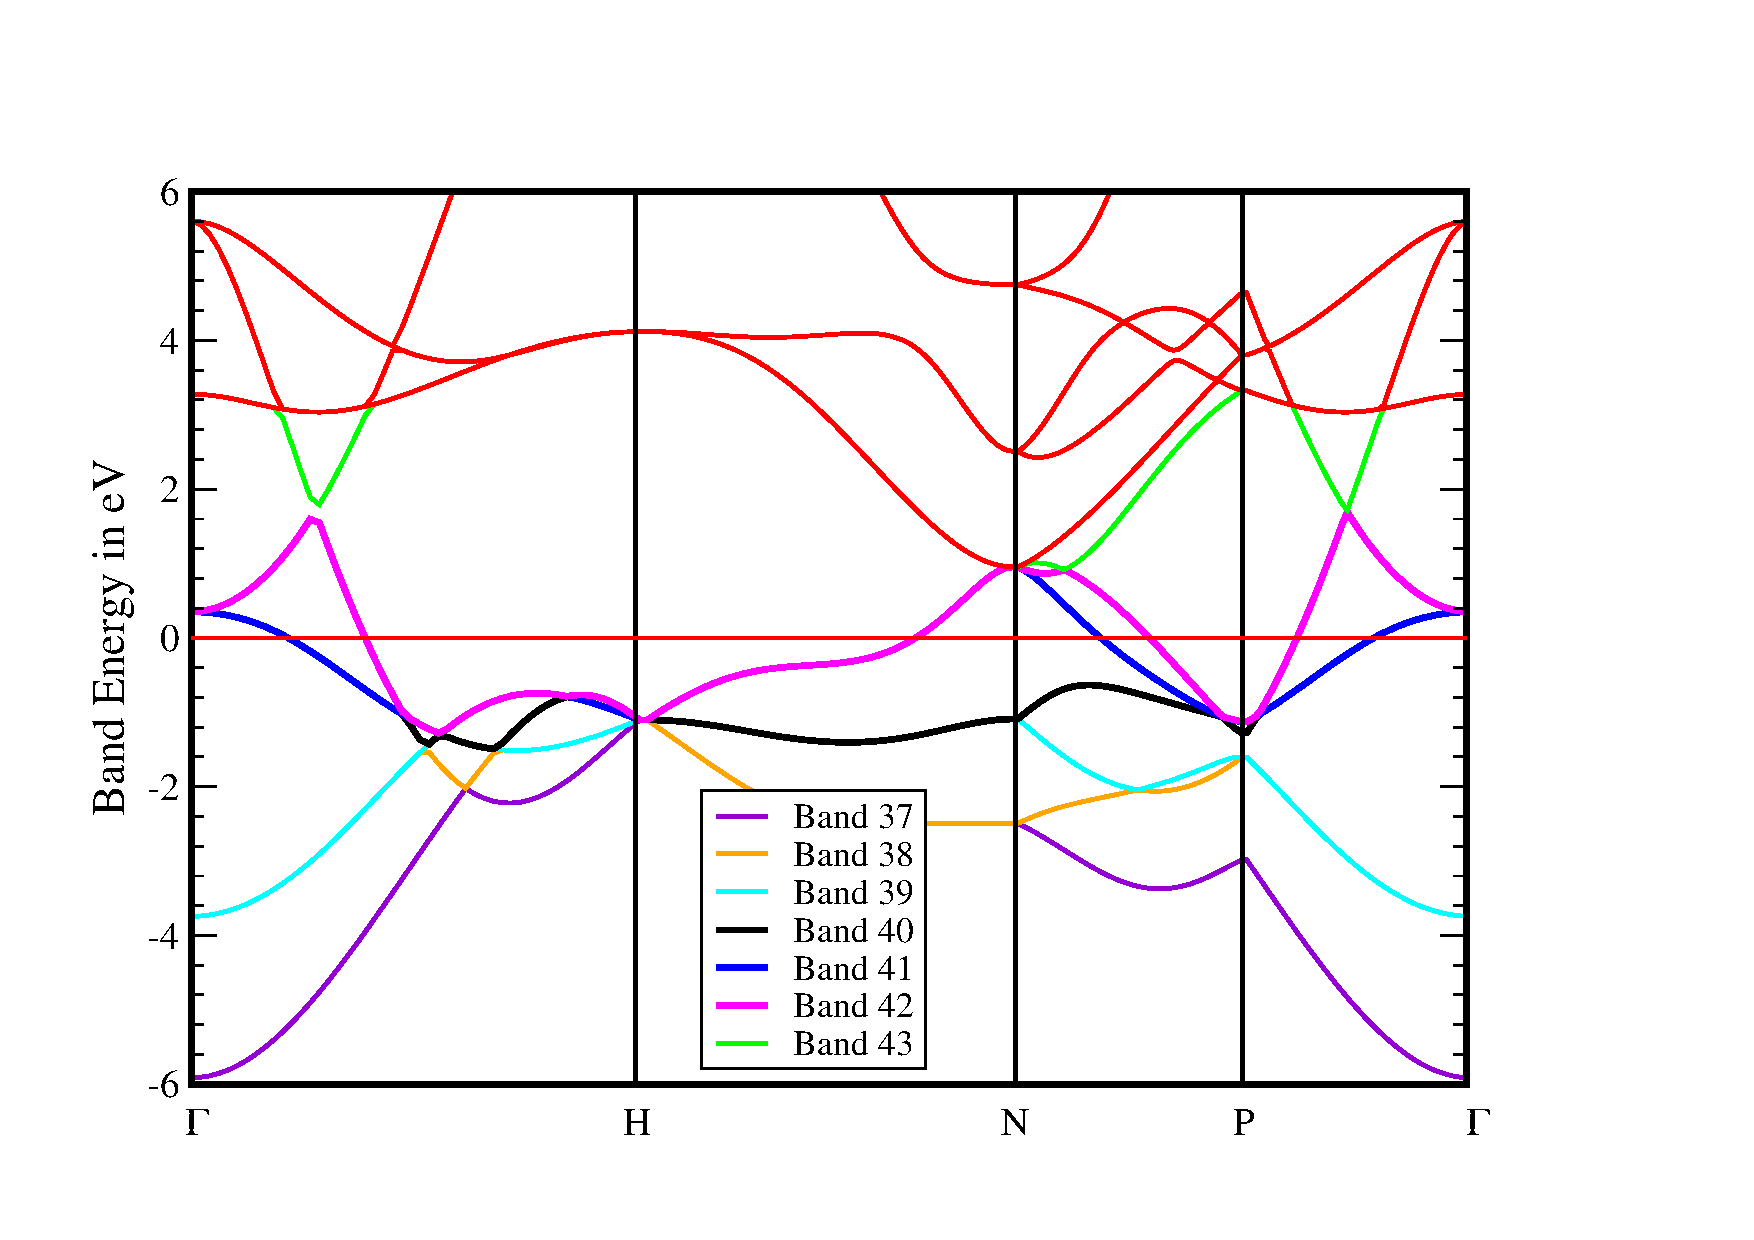
\includegraphics[width=0.74\textwidth]{bands-Nb.pdf}
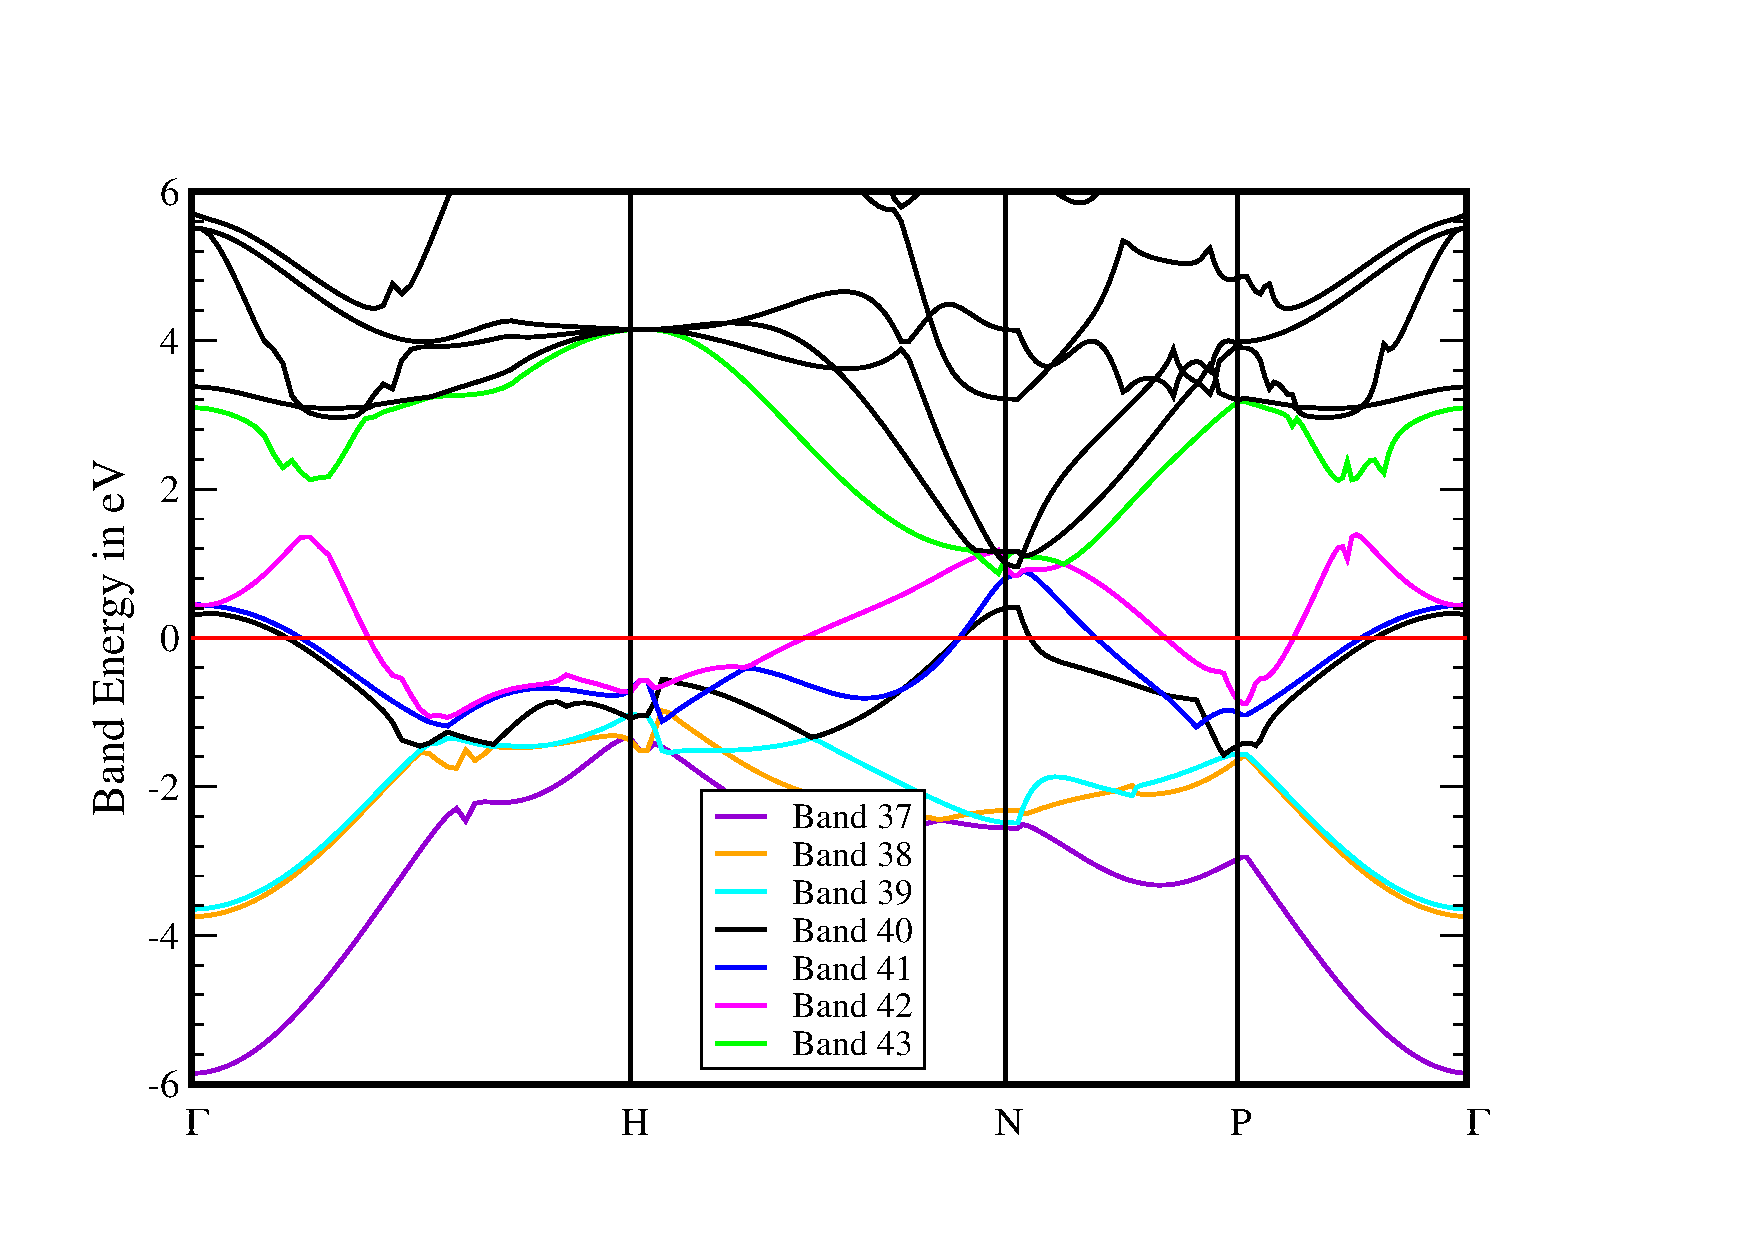
\includegraphics[width=0.74\textwidth]{Nb_bands_temperature.pdf}
\caption{\textbf{Temperature-dependent band structure and curvature in Nb.}
The temperature-renormalized band structure preserves coherent multi-band
connectivity and supports smooth curvature profiles, consistent with a stable
finite EDT regime.}
\label{fig:si_nb_temperature}
\end{figure}

\section*{S5. Curvature Topology Classification}

Beyond magnitude, the topology of curvature near degeneracies provides an
additional diagnostic for classifying electron--vibration coupling regimes.
Here curvature is defined with respect to a normal-mode coordinate and evaluated
along a momentum path~\cite{Giustino2017,Yarkony1996}. The goal of this
classification is not to replace the branch-resolved EDT-window extraction, but
to provide a higher-level geometric language for understanding why some
materials support broad, smoothly varying finite windows while others remain
sharper and more localized.

\paragraph*{Single-node curvature.}
In alkali and simple metallic systems, the curvature often exhibits a single
node or monotonic profile. This reflects relatively simple band dispersion and
limited mixing in the relevant subspace. In that case, the second-order
response changes sign at most once or remains one-sided, so there is little
evidence for a paired branch structure capable of supporting a stable local
quadratic manifold.

\paragraph*{Two-node smooth curvature.}
In systems such as Nb and K$_3$C$_{60}$, paired bands near the Fermi level
produce two nodes connected by smooth, approximately parabolic branches. The
curvature varies slowly across a finite region, allowing a consistent local
quadratic description and yielding a finite EDT window. This is the topology
most naturally associated with EDT-compatible behavior, because the curvature is
structured enough to indicate strong multi-band organization, yet smooth enough
to remain fit-compatible over a nonzero momentum interval.

\paragraph*{Two-node sharp curvature.}
In systems such as YBa$_2$Cu$_3$O$_7$ and LaH$_{10}$, two nodes can be present
but connected by sharply varying curvature with localized peaks. This rapid
variation prevents stable quadratic fitting despite strong coupling. The key
point is that strong electron--vibration response alone is not sufficient: if
the curvature changes too abruptly, the local manifold becomes too fragmented
to support a stable quadratic window.

\begin{figure}[p]
\centering
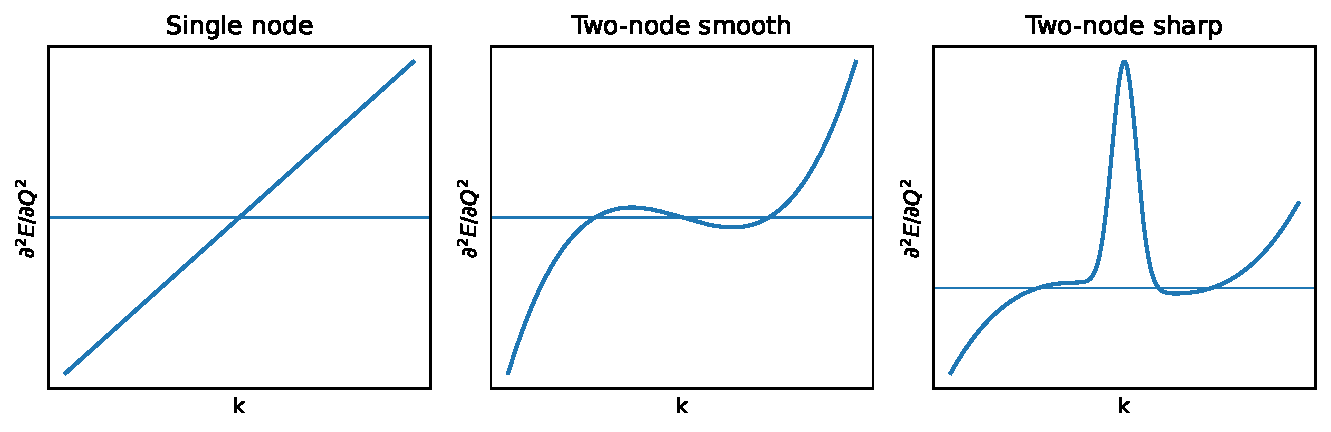
\includegraphics[width=0.95\textwidth]{figS7_curvature_topology.pdf}
\caption{\textbf{Schematic classification of curvature topology.}
Representative curvature profiles $\partial^2 E / \partial Q_\alpha^2$
illustrating three regimes: \textbf{left,} single-node curvature typical of
simple metals; \textbf{middle,} two-node smooth curvature with slowly varying
parabolic branches supporting a finite EDT window; and \textbf{right,} two-node
sharp curvature with localized peaks that suppress the formation of a stable
quadratic manifold. These classes are governed primarily by band dispersion and
lattice-scale parameters rather than pairing symmetry alone.}
\label{fig:si_curvature_topology}
\end{figure}

This topology view helps interpret the material atlas in Sec.~S3. The updated
Na and V selections occupy the single-node to smooth-two-node side of the
classification and therefore support broader or more stable extracted windows.
By contrast, the selected YBa$_2$Cu$_3$O$_7$ and LaH$_{10}$ subsets sit closer
to the sharp two-node regime, so their extracted windows remain more localized
even when a finite branch-resolved fit is still possible. In that sense,
Fig.~\ref{fig:si_curvature_topology} provides the qualitative geometric bridge
between the raw curvature traces and the quantitative $\Delta k_{\mathrm{EDT}}$
comparison reported earlier in the supplement.

\section*{S6. Plaquette Model and Trotter Circuit}

The minimal plaquette model used in the main text is
\begin{equation}
H =
J \sum_{\langle i,j\rangle} Z_i Z_j
+
h \sum_i X_i
+
\lambda Z_0Z_1Z_2Z_3 .
\end{equation}
This model isolates the ingredients needed for finite EDT dynamics: local
couplings, transverse control that enables operator spreading, and a loop term
that introduces nonlocal correlations. It is not presented as a quantitatively
fitted Hamiltonian for K$_3$C$_{60}$.

The reproducible implementation is the package \texttt{src/plaquette\_model}.
The Hamiltonian constructor is \texttt{build\_hamiltonian(J, h, lambda\_loop,
n\_qubits=4)}. Exact state trajectories, OTOCs, two-point correlations,
entanglement entropies, finite-regime scores, and Trotterized evolutions are
exposed by the same package.

\begin{figure}[p]
\centering
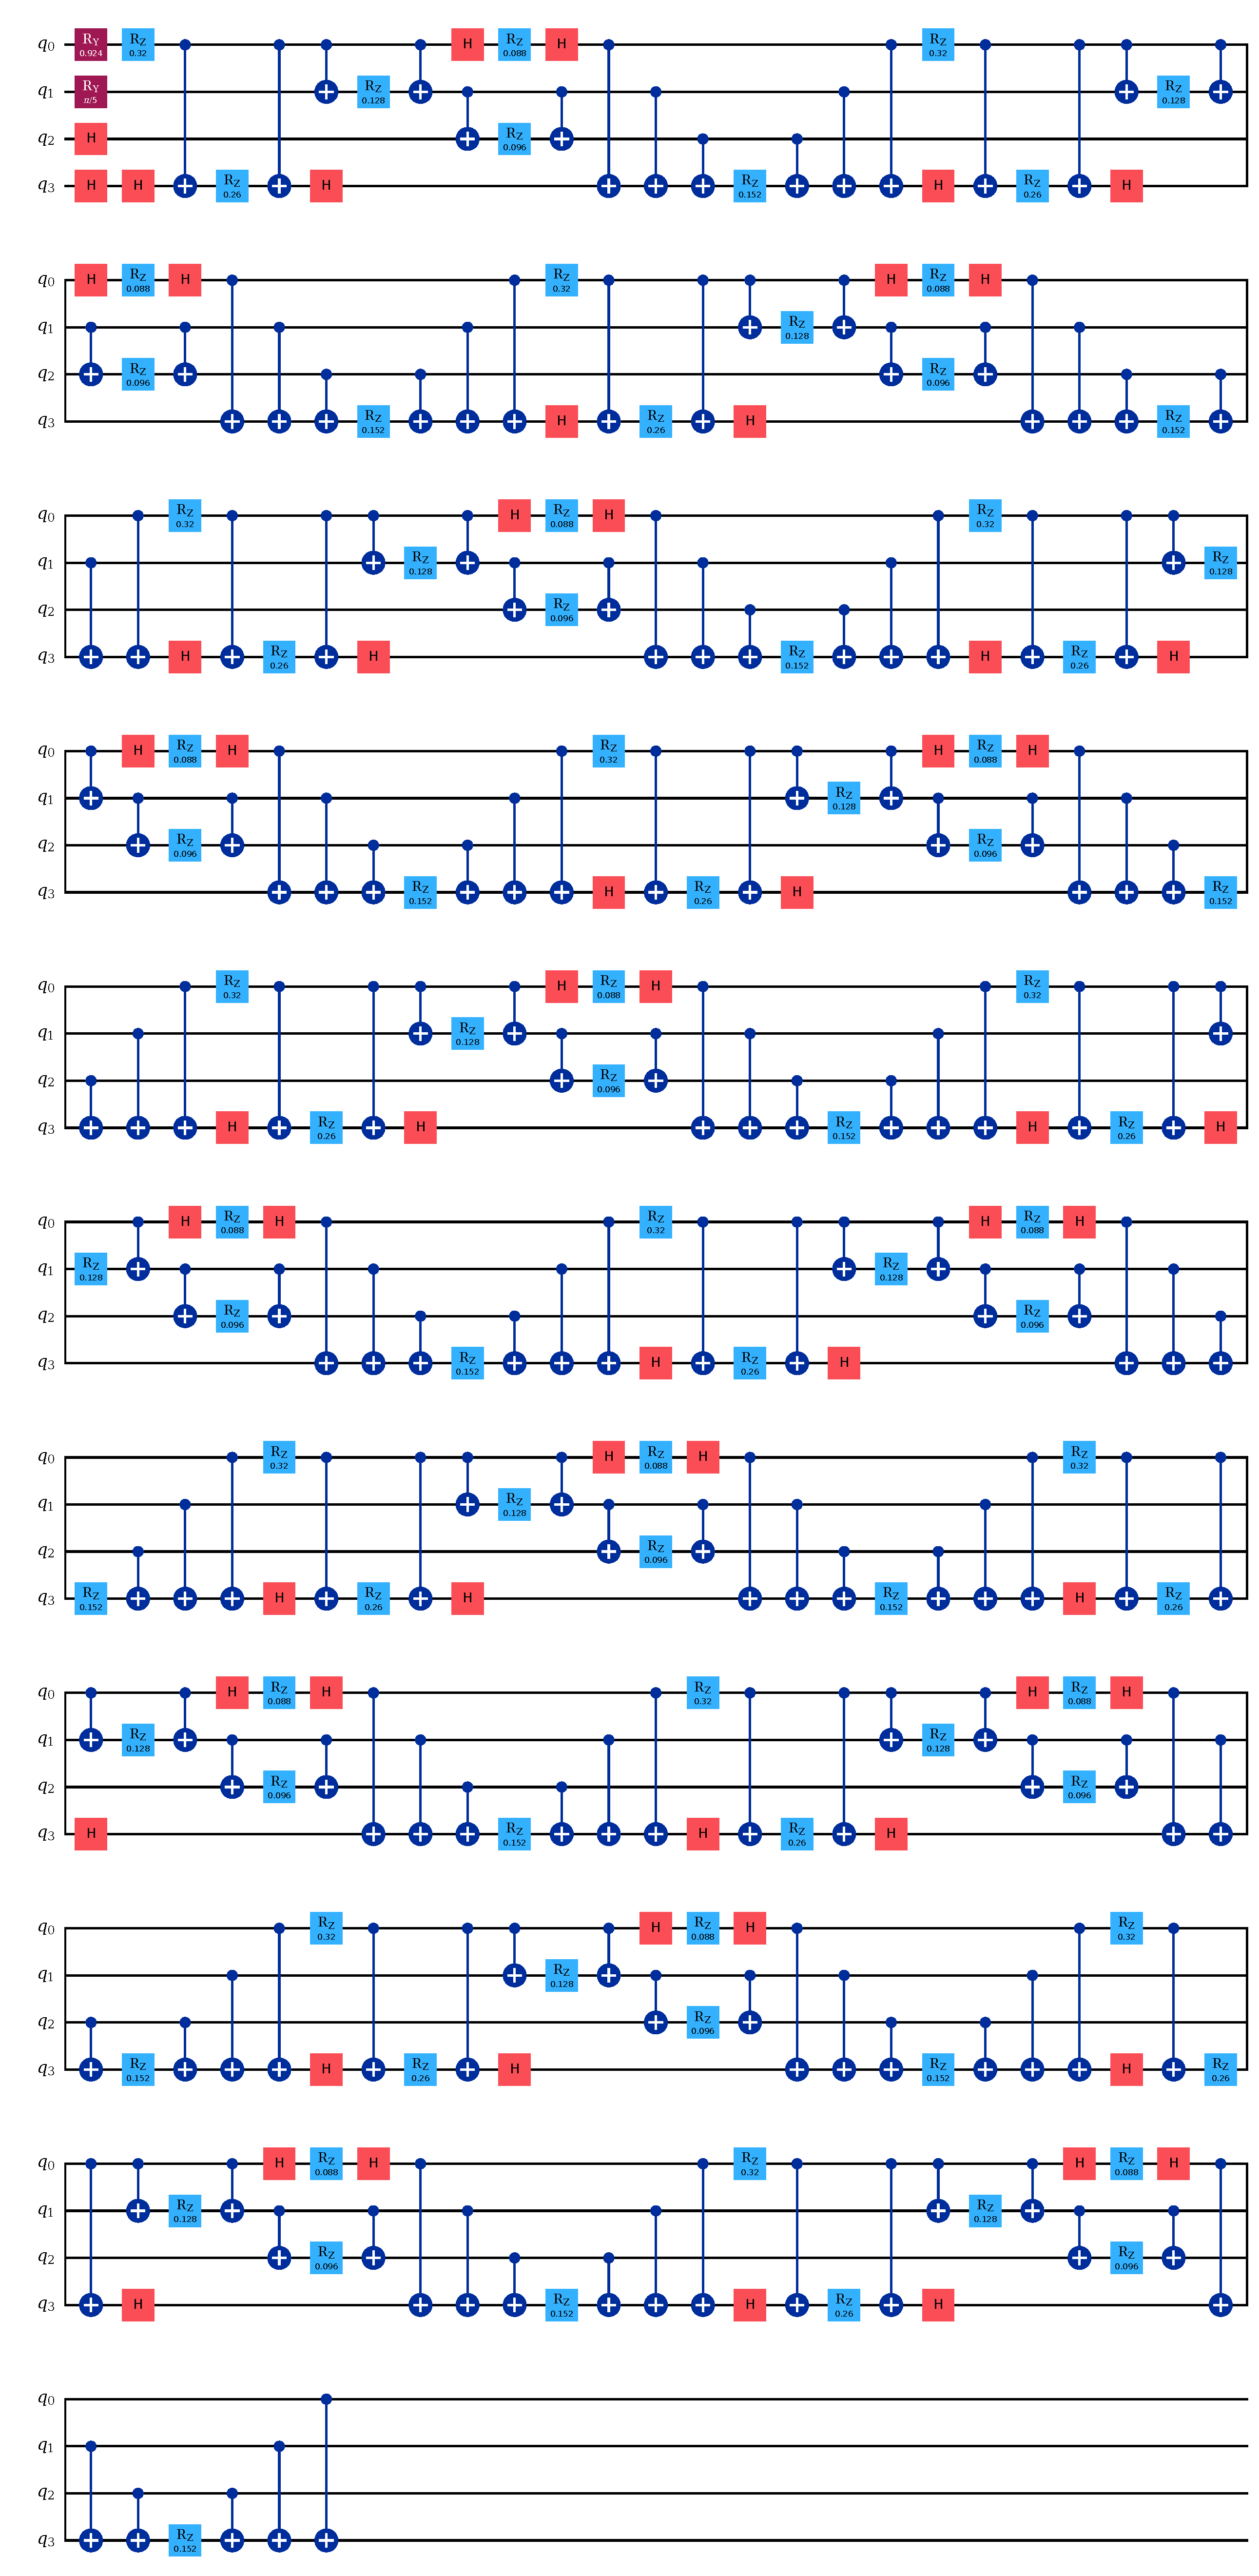
\includegraphics[width=0.58\textwidth]{demo_edt_gyro_trotter_4q_circuit_example.pdf}
\caption{\textbf{4-qubit plaquette Trotter realization of EDT dynamics.}
Representative first-order Trotter circuit for an archived plaquette-style
workflow. The plaquette unitary $e^{-i\lambda Z_0Z_1Z_2Z_3}$ generates
multi-qubit entanglement associated with loop topology.}
\label{fig:si_4q_plaquette_trotter_circuits}
\end{figure}

Time evolution under the minimal plaquette Hamiltonian is approximated using
first-order Trotterization, with circuit depth and gate count scaling linearly
with evolution time~\cite{Trotter1959,Suzuki1990,Lloyd1996,Childs2019}.
Observable errors are quantified by comparing exact and Trotterized expectation
values~\cite{BerryAhokasCleveSanders2007}. The finite dynamical regime is
characterized by sweeping $\lambda$ and identifying the optimum
$\lambda^\star$ that maximizes the dynamical EDT score.

\section*{S7. NV XY8 Model}

Quantum sensing in NV-center ensembles is analyzed within a quantum resource
engineering framework using a rate-based model~\cite{NVRateModel2023,Degen2017,Barry2020}.
For XY8 dynamical-decoupling sequences, the control parameter set is
\begin{equation}
\mathcal{C} =
\{P_{\mathrm{laser}},\, t_{\mathrm{read}},\, \Omega_{\mathrm{MW}},\,
\tau,\, N_{\pi},\, B_0,\, T,\, \mathrm{strain}\},
\end{equation}
which determines initialization, control, and environmental conditions of the
sensor~\cite{Casola2018}. These controls map onto an effective resource vector
\begin{equation}
\mathcal{R} =
\{R_{\mathrm{ph}},\, C,\, T_2(N_{\pi}),\, \chi(\omega),\, \mathrm{duty}\}.
\end{equation}
Here $R_{\mathrm{ph}}$ is the detected photon rate, $C$ is fluorescence contrast,
$T_2(N_{\pi})$ is the coherence time under dynamical decoupling, $\chi(\omega)$
is the filter-function response, and $\mathrm{duty}$ accounts for initialization
and readout overhead. The filter function is peaked near $\omega\simeq\pi/\tau$,
enabling frequency-selective amplification of ac fields~\cite{Cywinski2008}.

The sensitivity proxy is taken to scale as
\begin{equation}
\eta_{\mathrm{AC}}(\omega)
\propto
\frac{1}{\chi(\omega)C\sqrt{R_{\mathrm{ph}}T_2(N_{\pi})}}
\times f_{\mathrm{duty}},
\end{equation}
consistent with standard analyses of NV magnetometry sensitivity~\cite{Degen2017,Barry2020}.
Parameter sweeps over $(\tau,N_{\pi})$ identify finite optimal regimes set by
the competition between filter gain, coherence, pulse errors, and timing overhead.

\section*{S8. Reproducibility}

The reproducibility assets are organized in the repository root. The directory
\texttt{scripts/} contains figure-generation and analysis code, \texttt{data/}
contains bundled data products, \texttt{tests/} contains automated checks, and
\texttt{figures/} contains main and supplementary figure assets.

For K$_3$C$_{60}$, the main entry point is
\texttt{scripts/make\_fig2\_k3c60\_edt.py}. Running this script regenerates the
curvature panels used in the main-text K$_3$C$_{60}$ figure, the supplementary
robustness figure \texttt{figures/supplementary/S5\_threshold\_bootstrap.pdf},
and the summary file \texttt{data/k3c60/k3c60\_edt\_window\_summary.json}.

For the cross-material summary figure, the entry point is
\texttt{scripts/make\_fig1\_material\_summary.py}. Running this script
regenerates \texttt{figures/supplementary/S3\_material\_summary.pdf} via the
main figure asset and provides the compact width comparison used at the start of
Sec.~S3. The processed cross-material comparison table remains available in
\texttt{data/processed/material\_controls\_summary.csv}, and the broader common
scan figure can be regenerated with
\texttt{scripts/make\_figS4\_material\_controls.py}.

For the full replicated curvature-manifold material panels, the entry point is
\texttt{scripts/make\_material\_figure2\_panels.py}. Running this script
regenerates the Na, V, YBa$_2$Cu$_3$O$_7$, and LaH$_{10}$ panel sets in
\texttt{figures/supplementary/} together with the per-material summary files in
\texttt{data/processed/}.

For the plaquette-dynamics case study, the entry point is
\texttt{scripts/fig4\_plaquette\_dynamics.py}. It regenerates
\texttt{figures/main/fig4\_plaquette\_dynamics.pdf} and the processed sweep
table \texttt{data/processed/plaquette\_lambda\_sweep.csv}.

\section*{Summary}

Across the systems studied here, curvature arising from electron--vibration
interaction defines structured manifolds in which electronic states are
organized and degeneracies are lifted. The combined supplement documents the
normal-mode curvature calculation, the K$_3$C$_{60}$ finite-window algorithm,
the expanded curvature-manifold materials study, the plaquette-model
implementation, and the NV XY8 sensing model used to support the main-v4
manuscript.

\bibliographystyle{unsrt}
\bibliography{references}

\end{document}
